\documentclass[oneside]{report}

%Document Preamble
\usepackage[utf8]{inputenc}
\usepackage{graphicx}
\usepackage{float}
\usepackage{sectsty}
\usepackage[normalem]{ulem}
\usepackage{booktabs}
\usepackage{subfig}
\useunder{\uline}{\ul}{}

\graphicspath{{img/}}

\chapternumberfont{\LARGE} 
\chaptertitlefont{\Large}
\sectionfont{\large}
\subsectionfont{\normalsize}

\begin{document}
\begin{titlepage}

%----------------------------------------------------------------------------------------
%					LOGO SECTION
%----------------------------------------------------------------------------------------

\center

\includegraphics[width=8cm]{logo1.jpg}\\[1cm] % Include a department/university logo - this will require the graphicx package
 
%----------------------------------------------------------------------------------------

\center % Center everything on the page

%----------------------------------------------------------------------------------------
%				HEADING SECTIONS
%----------------------------------------------------------------------------------------

\textsc{\LARGE BSc Computer Science}\\[1.5cm] % Name of your university/college
\textsc{\Large Goldsmiths College, University of London}\\[0.5cm] % Major heading such as course name
\textsc{\large Department of Computing}\\[0.5cm] % Minor heading such as course title

%----------------------------------------------------------------------------------------
%				TITLE SECTION
%----------------------------------------------------------------------------------------
\makeatletter
\HRule \\[0.4cm]
\LARGE \textbf{LectureMate - Project Report}\\[0.4cm] % Title of your document
\HRule \\[1.5cm]
 
%----------------------------------------------------------------------------------------
%				AUTHOR SECTION
%----------------------------------------------------------------------------------------

\begin{minipage}{0.4\textwidth}
\begin{flushleft} \large
\emph{Author:}\\
Manpreet Singh Bance % Your name
\end{flushleft}
\end{minipage}
~
\begin{minipage}{0.4\textwidth}
\begin{flushright} \large
\emph{Supervisor:} \\
Golnaz Badkobeh \\[1.2em] % Supervisor's Name
\end{flushright}
\end{minipage}\\[2cm]
\makeatother

% If you don't want a supervisor, uncomment the two lines below and remove the section above
%\Large \emph{Author:}\\
%John \textsc{Smith}\\[3cm] % Your name

%----------------------------------------------------------------------------------------
%				DATE SECTION
%----------------------------------------------------------------------------------------

{\large June 2020}\\[2cm] % Date, change the \today to a set date if you want to be precise

\vfill % Fill the rest of the page with whitespace

\end{titlepage}

%----------------------------------------------------------------------------------------
%				DECLARATION PAGE
%----------------------------------------------------------------------------------------

\begin{declaration}
\addchaptertocentry{\authorshipname} % Add the declaration to the table of contents
\noindent I, Manpreet Singh Bance, declare that this report titled, \textbf{LectureMate - Project Report} and the work presented in it are my own. I confirm that:

\begin{itemize} 
\item Where I have consulted the published work of others, this is always clearly attributed.
\item Where I have quoted from the work of others, the source is always given. With the exception of such quotations, this thesis is entirely my own work.
\item I have acknowledged all main sources of help.
\end{itemize}
 
\noindent Signed:\\
\rule[0.5em]{25em}{0.5pt} % This prints a line for the signature
 
\noindent Date:\\
\rule[0.5em]{25em}{0.5pt} % This prints a line to write the date
\end{declaration}

\cleardoublepage

\tableofcontents
\newpage

\thispagestyle{empty}
\itemoffigures
 
\itemoftables

\newpage
\section*{Acknowledgements}

I would like to express my gratitude towards my supervisor, Golnaz Badkobeh, for her continued support and guidance throughout the course of the entire project, providing assistance from preparing the project for development to project completion.\\

I would also like to thank my family for their support in my studies throughout the duration of this degree.  \\

\par Finally, I would like to thank Lahcen Ouarbya, and the Department of Computing at Goldsmiths, University of London, for the opportunity to work on this project.

%----------------------------------------------------------------------------------------
%					 ABBREVIATIONS
%----------------------------------------------------------------------------------------

\begin{abbreviations}{ll} % Include a list of abbreviations (a table of two columns)

\textbf{MVP} & \textbf{M}inimal \textbf{V}iable \textbf{P}roduct\\

\textbf{CRUD} & \textbf{C}reate \textbf{R}ead \textbf{U}pdate \textbf{D}elete\\

\textbf{UI} & \textbf{U}ser \textbf{I}nterface \\

\textbf{API} & \textbf{A}pplication \textbf{P}rogramming \textbf{I}nterface

\end{abbreviations}

%-----------------------------------------------------------------------------------------------
%					INTRODUCTION
%-----------------------------------------------------------------------------------------------
\chapter{Introduction}
LectureMate is designed to be a cross-platform mobile application for use in an educational setting, namely, lectures - whereby, students and other academics can use the application to make dynamic, powerful and relevant notes which are linked to a specific timestamp or set of timestamps. The type of notes which can be made are rich text, uploaded images or camera photos, links, documents/research papers - all of which would the user would deem to be relevant to the point of the audio recording which is being made. As well as this, the user has the ability to highlight certain segments in the audio which they feel are important and they would benefit from later on when coming back to review these notes, for example, during revision.\\

As previously mentioned, the mobile app is mainly aimed at educators and academics in the educational setting but due to its capabilities could potentially be used in a range of other settings. Primary research showed that there were no existing applications on the market which offered the functionality that this mobile application aims to do. Existing applications such as Evernote are based primarily on text-based notes with the ability to add further attachments, whereas LectureMate would be audio-based allowing for notes to be made based on the timestamp in the audio recording.\\

Secondary research was able to prove that educators (the primary target market) and among students at Goldsmiths College, University of London, that there was no one consistent form of making clear, relevant notes and that the target market relied on a number of various applications to make notes which was not a practical solution. These applications incliuded the likes of Evernote, Microsoft OneNote, Google Docs, as well as traditional notes which were made with pen and paper which were later difficult to merge with existing notes on these applications.\\

Research was carried out to look at the usage of smartphones and devices for carrying out activities in day-to-day life which showed that a multitude of things were done illustrating that the application would be a good fit for carrying the task the application solves. \textbf{[9]}\\

As well as this, I also looked the number of smartphone users in the UK and whether this number was likely to increase in the UK, \textbf{[8]}, to which the results showed that this number would increase rapidly and somewhat plateau meaning most people would own one. Again, this proving that the application being both available on both platforms as well as a mobile application would be a more than satisfactory solution.\\

From this, it was clear that the application would aim to provide a satisfactory solution to the needs of the market and honoring what is in need by the target market which was able to be identified through the research. As a result, upon deployment of the application we would be able to see whether this is fulfilled and is versatile enough to meet the needs of its users. This is evidence to show how an application and platform such as LectureMate is vital in filling a much needed gap in the market.

	\section{Motivation}
The motivation behind this mobile application is upon research the lack of platforms which allow users to make notes based on audio recordings. As well as this, in first-hand experience, I was able to identify that I found note-taking particularly inconsistent and upon coming back to these notes to revise I found these notes to have no context and difficult to understand. Therefore, I carried out some research to see whether any platforms existed which allowed notes to be made but with some context and found that there were none for wide use.\\

By this and by communicating with peers among different educational settings, I was able to recognise that most universities and lecture theatres had recording equipment. I initially upon ideation, thought of pursuing this, however, later came to the conclusion that this would not be a viable option due to the issues with obtaining the permission of those individuals who may be visible in the recording, and as a result I made the final decision to proceed with the same idea however, using audio recording instead.

	\section{Scope}
LectureMate aims to combat the issues that students and academics face in the note-taking and revision aspect of their learning by providing a platform where they can make clear, dynamic and consistent notes in order to tackle the existing problems faced with making notes where the notes are made across different platforms making them different to compile and are inconsistent. Therefore, making clear, consistent and dynamic notes using LectureMate are a solution to these issues.

	\section{Objectives}
One of the first things which were looked at was how I can meet the objective to fulfill the need for the target market which was identified. LectureMate does this by providing a platform to satisfy the need for making clear notes.\\

I needed to make sure that the application met the needs that my target market fed back to us when conducting our primary and secondary ressearch. Another objective that was indicated through executing this research was that the application would have the ability to highlight specific points within the audio where upon reviewing, would be able to identify the key, relevant sections of a lecture or recording.\\

The security and integrity of the notes which are made are a priority as these notes are to be kept safe whereby unauthorised changes should not be made to the notes as well as their security being ensured as to them not becoming deleted or corrupted. Therefore, considering this, the app aims to be a safe and reliable platform for its users so that they do not need to worry about the integrity of their notes. The application will do this by saving the note as a file in a folder creating regular backups each day or manually.\\

As the files will be stored locally on the device, the user is responsible for any data which might be subject to any tampering or corruption to the files when being manipulated through any third party application such as a file explorer. Using the application to make any changes to any notes will be a tested and safe way for users to alter notes.

\chapter{Technical Specification}
	\section{Background Research}
	Here, I will focus and discuss the research I carried out prior to commencement of the design of the application. I will begin technical research looking at the potential for technologies I may use to develop the mobile application and briefly address the reasons behind this.

		\subsection{Existing Systems}
In the research stage, I wanted to explore the market for existing applications which perform or complete similar or exactly the functions that I was aiming for in this application. I decided to look at features I would be able to implement from others or simply known, working models which wre proven to be good applications and have relevant, useful features I could also implement. However, I wanted to be inspired by these and not just implement the feature in the same way as the app I would be borrowing from.
			\subsubsection{Soundcloud}
While carrying out research, I thought of existing systems which I can obtain certain features from which I might be able to incorporate into the mobile application. Soundcloud came to mind whereby in their interface, they have the ability to allow their users to add comments at certain time points in the audio which had been uploaded. I thought this same model could be applied to my application as notes can be added at a specific point in the audio recording.
			\subsubsection{Evernote}
Again, whilst looking at existing applications, Evernote who provide a cross-platform note taking solution. I therefore studied this application well and listed features I also look to implement into my application - these included: the ability to upload images, audio attachments and links. These features would all be very useful in a note taking setting, especially in a lecture setting.

	\section{Overview}
The technical architecture of the mobile application is as simple as the layering mode. The logic of a layered architecture allows the separation of the Front-End, Middleware and Back-End, however still allowing for cohesion between these, which will be detailed further.\\

The uppermost layer will be the presentation layer - which will be the appearance and interaction side of the application, the middle layer - which will be responsible for the (business) logic behind the application containing the code behind the actions interacted with in the presentation layer, and the data access layer - which will be the back end code which enables the user to access and make changes to the notes, although stored locally, they will still carry out CRUD functionality similar to that used in databases.

	\section{Application Frameworks}
A framework is an abstraction where software is written to provide generic function to achieve a task or tasks. This mobile application has made use of some frameworks to contribute to the functioning of it - mainly being in the Front-End or 'Presentation Layer'.

	\section{Full Stack Development}
As previously mentioned, the web application was designed and structured in a way conforming to the stack structure: Front-End, Middleware, and Back-End. This section will further discuss the specification of technologies in each tier of the stack and the reasons behind their uses: 

		\subsection{Flutter}
The entirety of the mobile application will be using the existing Flutter framework which is an open-source UI software development kit created by Google - used to develop applications across mobile, web and desktop applications. I will detail the framework architecture and the way each of these are used in the development of the mobile application: 

		\subsubsection{Dart platform}
Flutter apps are written in the Dart language and make use of many of the language's more advanced features. The Dart language package allows during development for implementing features into the application which help shape the appearance and layout as it appears to be.\\

During the development stage, the Dart package also allows for dynamic and a live coding experience which involves hot reloading whereby any changes in code can be updated and made live without having the whole application have to be restarted for the new changes to take effect which was a welcome and proven helpful feature to the process.

		\subsubsection{Flutter engine}
The flutter engine provides low-level rendering support interfacing with iOS and Android platforms which hosts the Fluttter applications and manages the way they look and behave controlling and making use of its core libraries which include animation and graphics, file and network I/O, accessibility, plugin and runtime and compilation toolchain. However, these were things which during the development process were something which were not deeply explored and only utilised for basic functionality.\\

Using the Flutter framework allowed for a more reactive, modern framework for creating a modern and engaging mobile application which would also function well.

		\subsubsection{Foundation library}
The foundation library written in Dart allowed for the use and implementation of basic classses and functions in the mobile application enabling access to APIs to communcate with the engine and construct the application.

		\subsubsection{Widgets}
Flutter widgets are built into the package and work as the different components which make up together to build the application, such as buttons and text. These are included as standard and are used in the application for some of the components.\\

Design-specific widgets such as Material design using Google's design language as well as Cupertino which use Apple's Human Interface Guidelines iOS design, both make use of these respective design langauges to display the application best in their respective, native environments to give them a more uniform look despite being on different platforms.
	
		\subsubsection{Google Firebase}
At a later stage in the implementation stage, it was concluded that issues would arise with the storage and retrieval of data, namely media such as images, videos and audio as it would be difficult to reference in using the application and it made sense to make use of a database to solve this. Due to the nature and cohesiveness of Google developed systems, it would make sense to use Google Firebase as the database management.\\

This would allow for the storage of raw data such as strings and numerical characters; Firebase also has a solution for the storage of media items as this utilises Firebase storage which gives each record a unique identifier which can be associated to the respective note and would could be stored successfully.

%-----------------------------------------------------------------------------------------------
%					PROJECT MANAGEMENT
%-----------------------------------------------------------------------------------------------
\chapter{Project Management}

	\section{Resource Management}
Prior to commencement of the project, I planned to allocate resources in the form of time, being the number of hours spent, on each stage of the project with ideation to conception, research, development and testing stages to ensure that this was all done in good timing and enough resources were spent on each stage so that it would be produced to a high standard. Following the allocation of resoruces available throughout the project, I created a timeline with set provisional dates whereby these tasks should be completed, referred to as milestones.

Taking this approach to the allocation of labour and resources means I can plan when certain tasks should be done and if these are not met, I can allocate further resources to make the project less susceptible to interruptions, which may include:

\begin{enumerate}
\item \textbf{Overlap of tasks:}\\
The tasks were divided in smaller segments to ensure better productivity and efficiency in completing each tasks and to make sure that each task was completed correctly prior to moving onto the next task. This guaranteed that there was less of a feeling of  being stuck on a particular task for a prolonged amount of time and a wider variety to provide a faster workrate of tasks being completed. Due to the nature of the developmemt process being in Flutter, the bulk of the project was the middleware and backend controlling the way functions and features were supposed to behave and whether these were being suitably met. The tasks were divided in such a way that there was no dependency of completion of a task to complete the next as such until it came to testing to see whether these worked together cohesively.
\item \textbf{Time keeping and meeting deadlines:}\\
The time keeping and milestone aspect of the planning process was very important so that each of these were being met on time and no stage of the development process was falling behind so much so that it would not be complete and the application as a whole would suffer. To combat this, I created a blog so that I was keeping track of the developments made in the project each week to track whether this progress was good and steady and would meet the milestones at the correct times. Planning these milestones enables for a greater control of the project and the way it is progressing.
\end{enumerate}

	\section{Gantt Chart}
	I utilised a Gantt Chart to plan and make efficient use of my time to make sure I was making good progress and tracking milestones to monitor whether these were being met on time and/or if I needed to deploy more resources elsewhere to ensure a timely finish to a good standard. The Gantt chart can be seen in \textbf{Appendix F}.

	\section{Methodology}
		\subsection{Agile Development Method}
The Agile Project Management Methodology was utilised where, by definition, an iterative process made use of at each stage of development in all areas of the development stack requiring constant effective communication. Using the Agile method meant that the project was dealt with the most efficient way possible with larger tasks being broken down and divided as to the larger and smaller tasks taking varying time to complete and complete these tasks effectively.

		\subsection{Kanban}
The Kanban method is also used in order to keep track of the items which need to be completed and which are still yet to be completed as well as a section to review code and carry out ah-hoc testing as well as component testing to see whether each component is working as expected. This also provides a more broader look at the tasks to come and time to prepare for these, seeing whether any previous tasks are dependant or feed into the following task. The Kanban method is visualised using Trello.

	\section{Version Control}
		\subsection{Git}
The project makes strong use of Git and its features for version control purposes, with the ability to see and track any changes to files and have a history of the previous changes made and to apply any future fixes giving more of a sense of control and responsibilty for each task to be completed correctly as well as the a timestamp of when this has been completed to identify whether it has been done in good time according to the milestones and personal proposed dates.

%-----------------------------------------------------------------------------------------------
%					ANALYSIS
%-----------------------------------------------------------------------------------------------
\chapter{Analysis}
	\section{System Requirements}
	System requirements outlines the criteria needed to complete the application to a standard meeting the MVP and beyond. This is looked at in two separate sections, functional and non-functional requirements. These requirements are set here so as to build and define clear terms to avoid any misunderstanding in any of the stages of implementation which in turn allow me to predict the challenges I might face and be ready to spend more time and allocate resources here whereby I can plan time spent on each stage to clearly visualise a viable and realistic application to produce in the timeframe and to what standard I can produce this to.\\

Essentially minimum requirements the application are expected to handle and accommodate:
		\newpage
		\subsection{Functional Requirements}
		\begin{table}[H]
			\begin{tabular}{|l|l|l|}
			\hline
			ID   & Description                                                                                                                                                             & \begin{tabular}[c]{@{}l@{}}Vital/Optional \\ 						Requirement\end{tabular} \\ \hline
			FR01 & Mobile application to run at least on all Android devices                                                                                                               & Vital                                                                 			\\ \hline
			FR02 & \begin{tabular}[c]{@{}l@{}}Mobile application requires constant, reliable access to internet \\ connection to user's device\end{tabular}                                & Vital                                                                 			\\ \hline
			FR03 & \begin{tabular}[c]{@{}l@{}}Mobile application user input data to be stored securely on \\ Google Firebase\end{tabular}                                                  & Vital                                                                 			\\ \hline
			FR04 & \begin{tabular}[c]{@{}l@{}}Mobile application to back up audio recordings to be stored \\ locally on device in the event of unreliable internet connection\end{tabular} 			& Optional                                                              \\ \hline
			FR05 & \begin{tabular}[c]{@{}l@{}}Mobile application should allow the user to make notes and be \\ able to retrieve and view these\end{tabular}                                & Vital                                                                 			\\ \hline
			FR06 & \begin{tabular}[c]{@{}l@{}}Mobile application should enable the user to carry out CRUD \\ functionality through the database\end{tabular}                               & Vital                                                                 			\\ \hline
			\end{tabular}
			\caption{Functional Requirements}
			\label{Functional Requirements}
		\end{table}

		\subsection{Non-functional Requirements}
		\begin{table}[H]
			\resizebox{\textwidth}{!}{
			\begin{tabular}{|l|l|l|}
			\hline
			ID   & Description                                                                                                                                                             & \begin{tabular}[c]{@{}l@{}}Vital/Optional \\ 						Requirement\end{tabular} \\ \hline
			NFR01 & Mobile application should run on Android or iOS mobile device & Optional                                                                 			\\ \hline
			NFR02 & \begin{tabular}[c]{@{}l@{}}Mobile application should be usable easily for any user to achieve \\the purpose of the application\end{tabular}                                & 					Vital                                                                 			\\ \hline
			NFR03 & \begin{tabular}[c]{@{}l@{}}Mobile application should store the data with integrity without the \\ability to maliciously alter data\end{tabular}                                                  			& Vital                                                                 			\\ \hline
			NFR04 & \begin{tabular}[c]{@{}l@{}}Mobile application should have all features working as expected \\without any bugs\end{tabular} 			& Optional                                                              			\\ \hline
			NFR05 & \begin{tabular}[c]{@{}l@{}}Mobile application should perform all actions without significant delay \\within reasonable time period of no more than 10 							seconds\end{tabular}                                & Vital                                                                 			\\ \hline
			\end{tabular}}
			\caption{Non-functional Requirements}
			\label{Non-functional Requirements}
		\end{table}

	\newpage
	\section{Stakeholders}
	Stakeholders are those with an interest in the subject - which in this case is the mobile application. As previously mentioned, the aplication is targeted for those in educational settings including students and academics but can also be used for various functions outside this setting. \\
	
	Taking this into consideration, the application can be used by people of all ages, however, more than likely those over the age of 18 but is not limited to this. With this assumption in mind it made sense to carry out a survey to see whether this was assumption could be proven true or disproved which is of great importance so the specification of the application can be modified accordingly.
	\newpage
	\section{Use Case}
	A use case diagram is a illustrated display of intercommunication between users or parts of a system which shed light on the requirements of the system and the role each component plays in order to achieve a successful product/outcome.

%-----------------------------------------------------------------------------------------	
		\subsection{Use Case Diagram}
		\begin{figure}[H]
			\begin{center}
	 		 	\makebox[\textwidth]{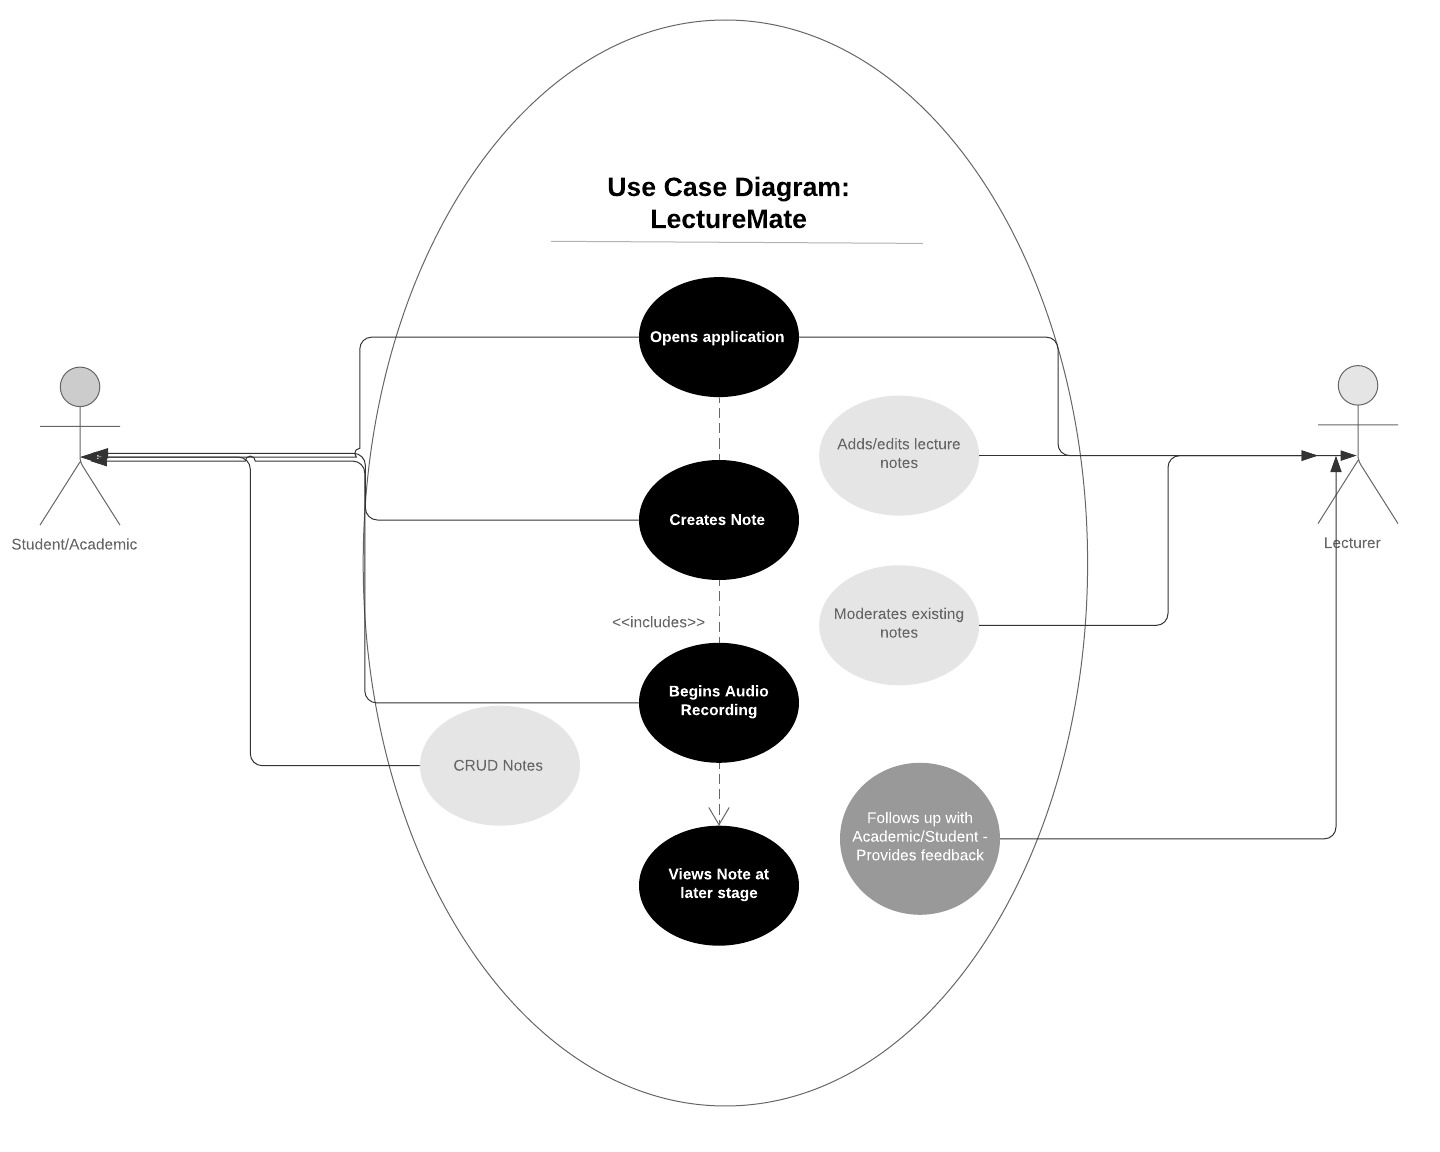
\includegraphics[width=6in]{/UseCase_UML.jpeg}}
			\end{center}
			\caption[Use Case Diagram]{Use Case Diagram}
		\end{figure}

%-----------------------------------------------------------------------------------------	

		\subsection{Use Case Scenarios}
		These scenario's will give a brief understanding as to the uses of the application by its potential users. These were designed to be aimed at the Student/Academic, and the Lecturer as will be detailed below.
		\newpage
			\subsubsection{Student/Academic - Creating a new note}
			The Student/Academic will use the application to make notes as per its purpose in a lecture, whereby they will open the application, which will load to the home screen giving the user the option to create a new note which upon clicking will display the New Notes page as can be seen in \textbf{Figure 4.1} below:

		\begin{figure}[H]
			\begin{center}
	 		 	\makebox[\textwidth]{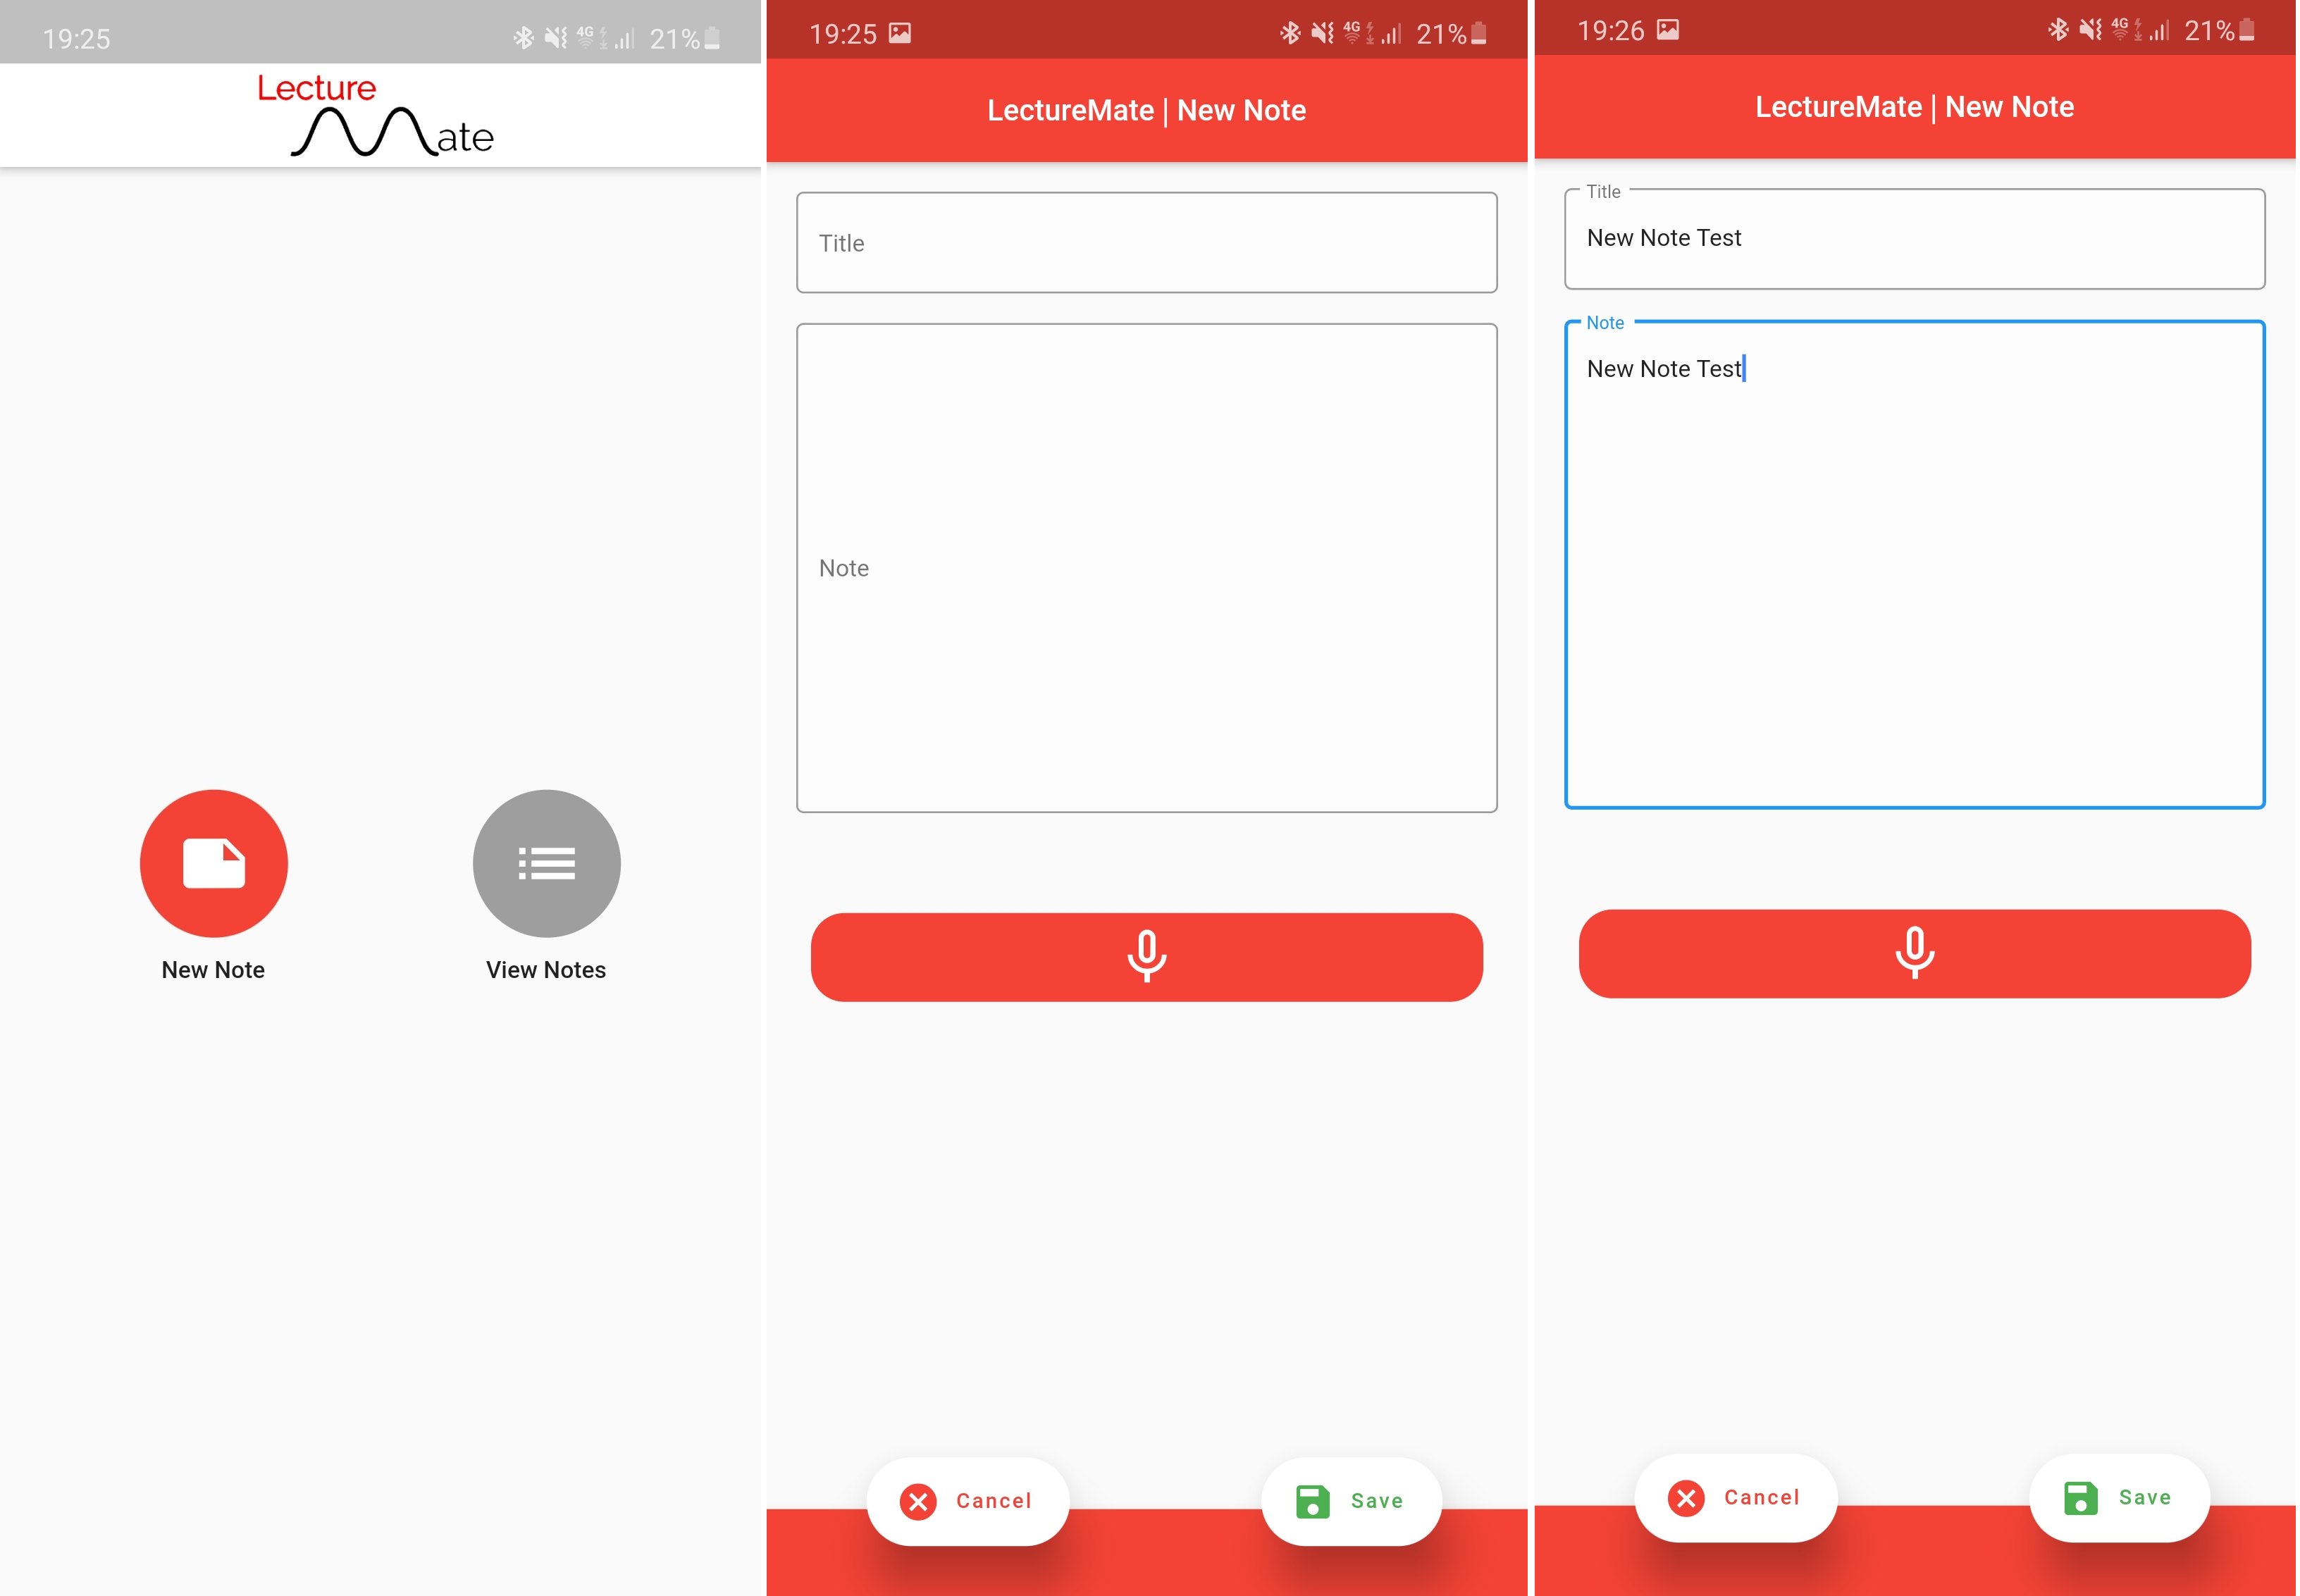
\includegraphics[width=6in]{/newnote_process.png}}
			\end{center}
			\caption[New Note Process]{New Note Process}
		\end{figure}
		\newpage

%-----------------------------------------------------------------------------------------
			\subsubsection{Student/Academic - Revising (reviewing notes)}
			When the user will come back to review notes potentially for revision purposes, they can do this by visiting the View Notes section of the application which displays all the cards which they have previously entered.\\

Following this, they can read the notes from the card itself and play the audio appended to the note by clicking the 'LISTEN' button and go back to the note with the recording still playing in the background.\\

The process is demonstrated below in \textbf{Figure 4.2}:

		\begin{figure}[H]
			\begin{center}
	 		 	\makebox[\textwidth]{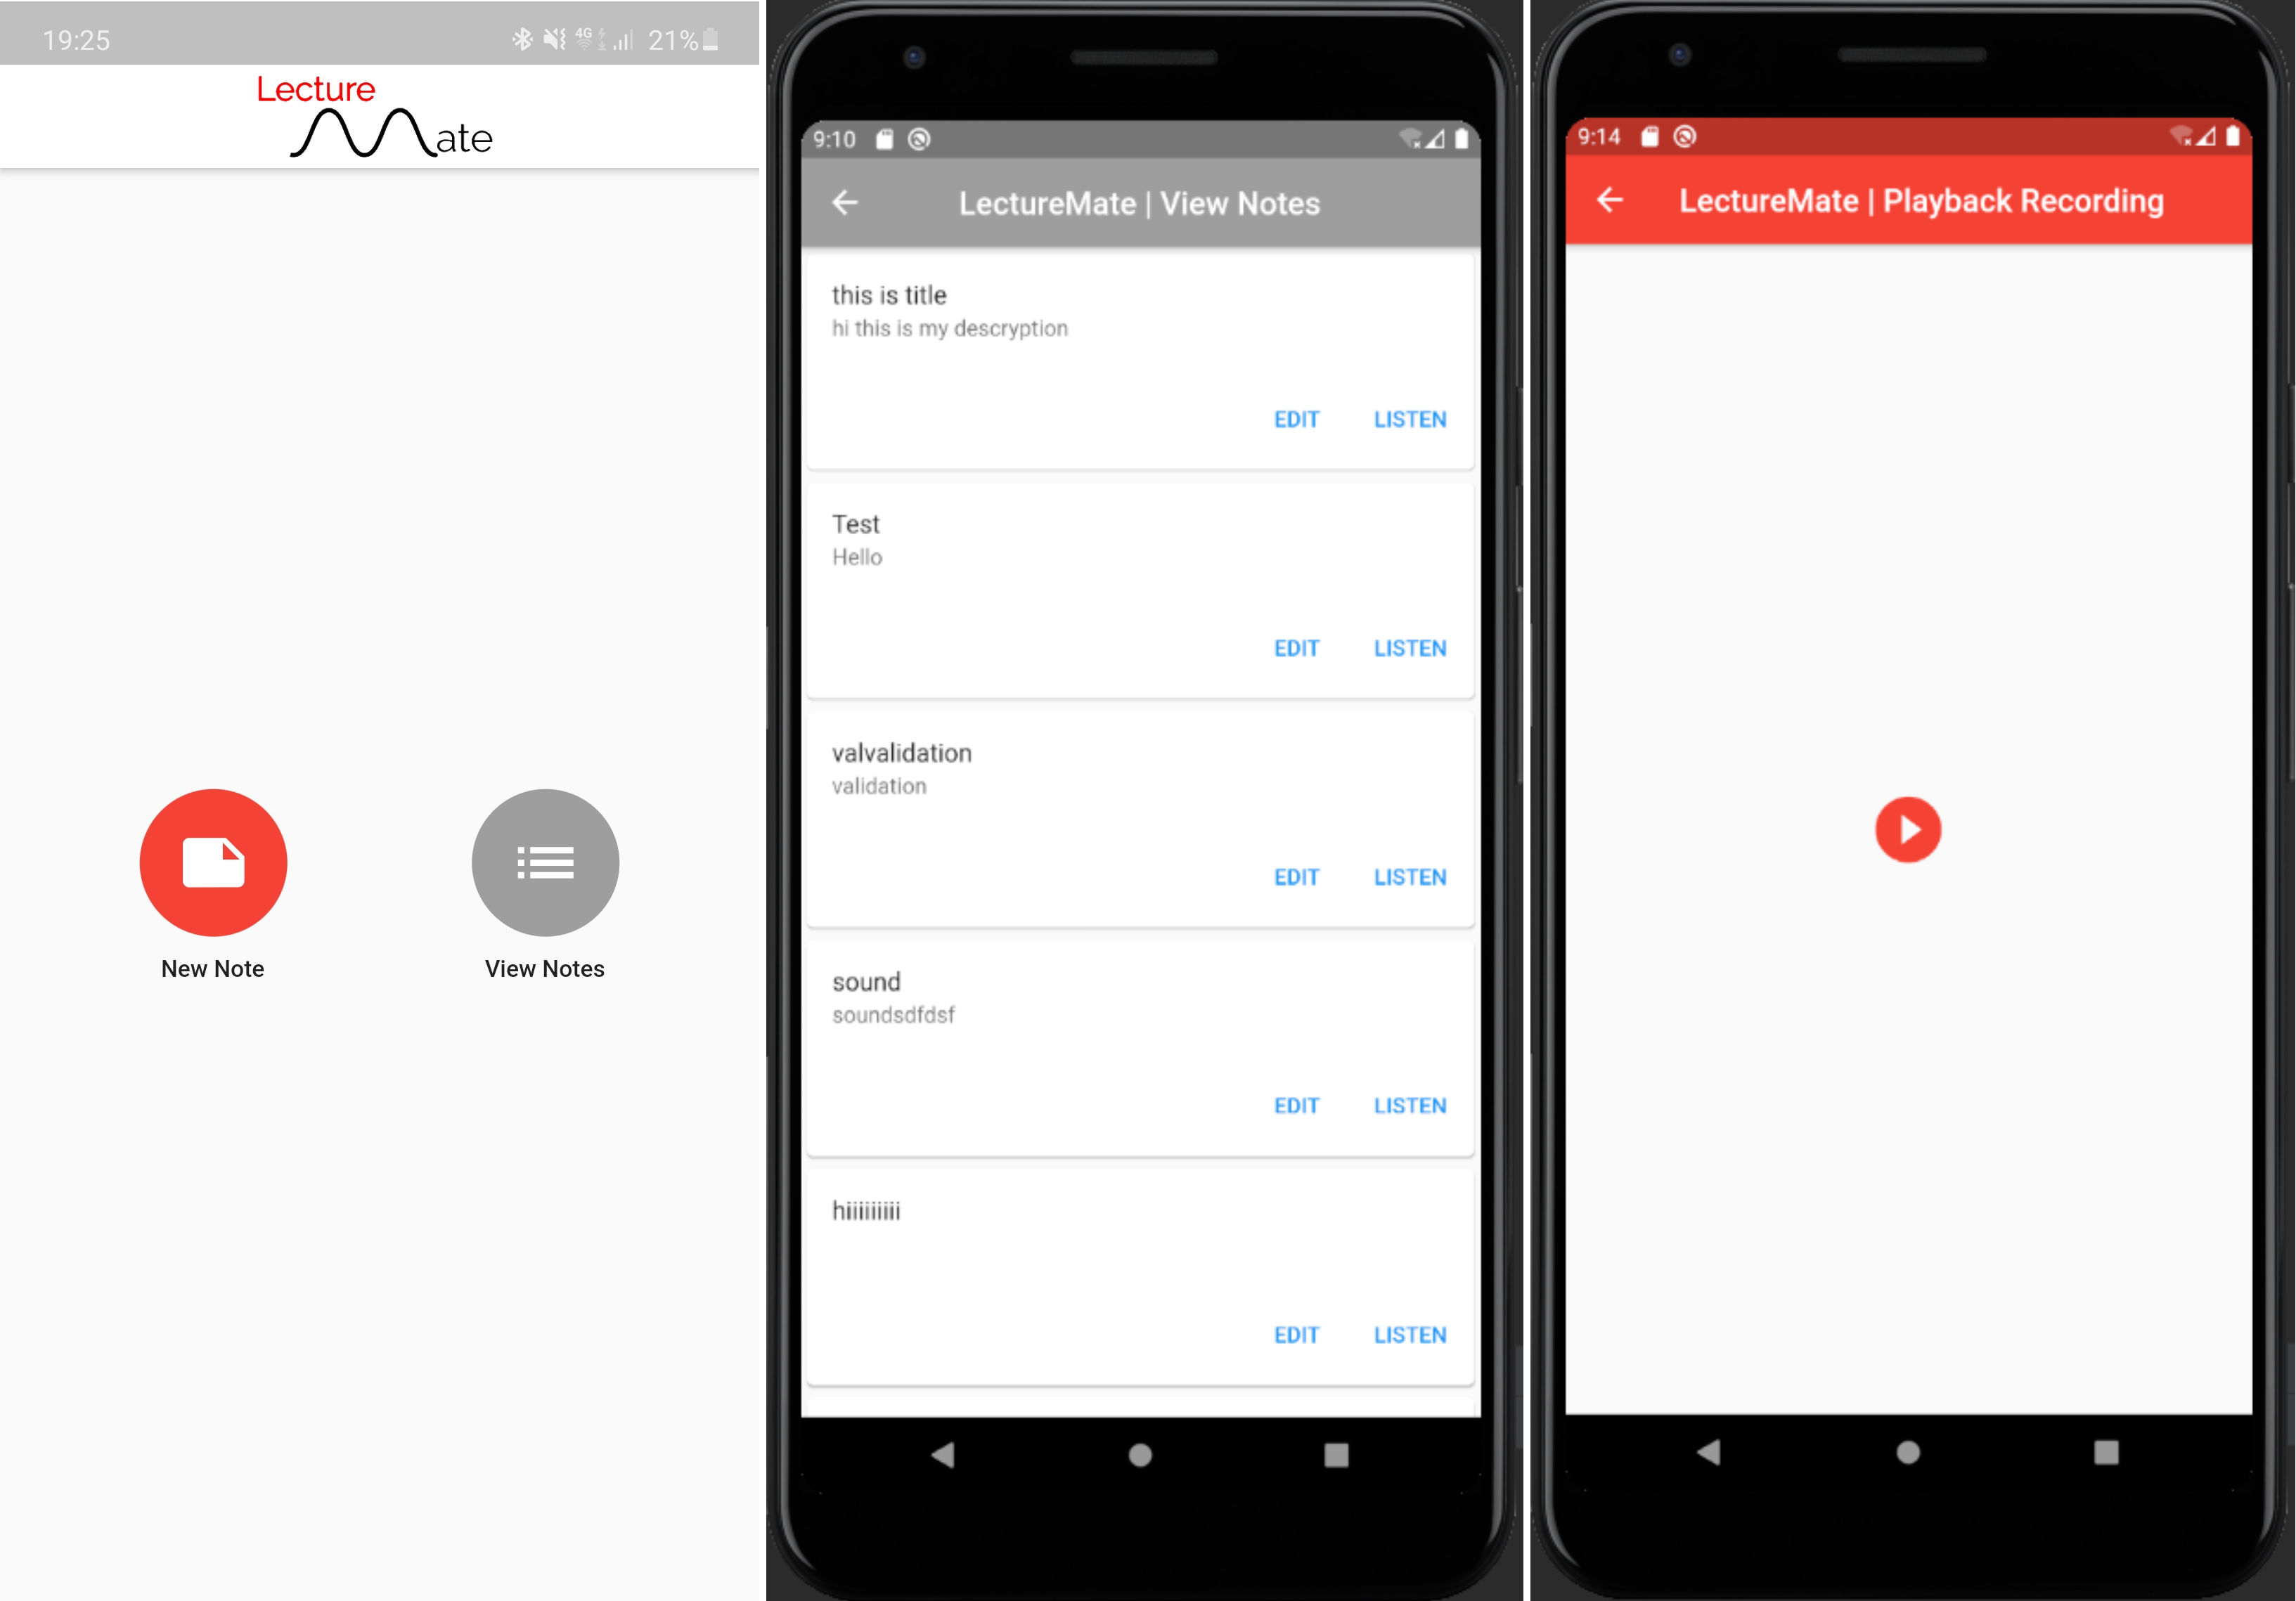
\includegraphics[width=6in]{/review_process.png}}
			\end{center}
			\caption[Review Note Process]{Review Note Process}
		\end{figure}
		\newpage

%-----------------------------------------------------------------------------------------
			\subsubsection{Lecturer - Editing notes}
			A lecturer would use the application for the purpose reviewing the notes made by students and see whether these are correct, any changes that would need to be made can be done by editing the concerning note. The process can be seen as displayed in \textbf{Figure 4.3} below:

		\begin{figure}[H]
			\begin{center}
	 		 	\makebox[\textwidth]{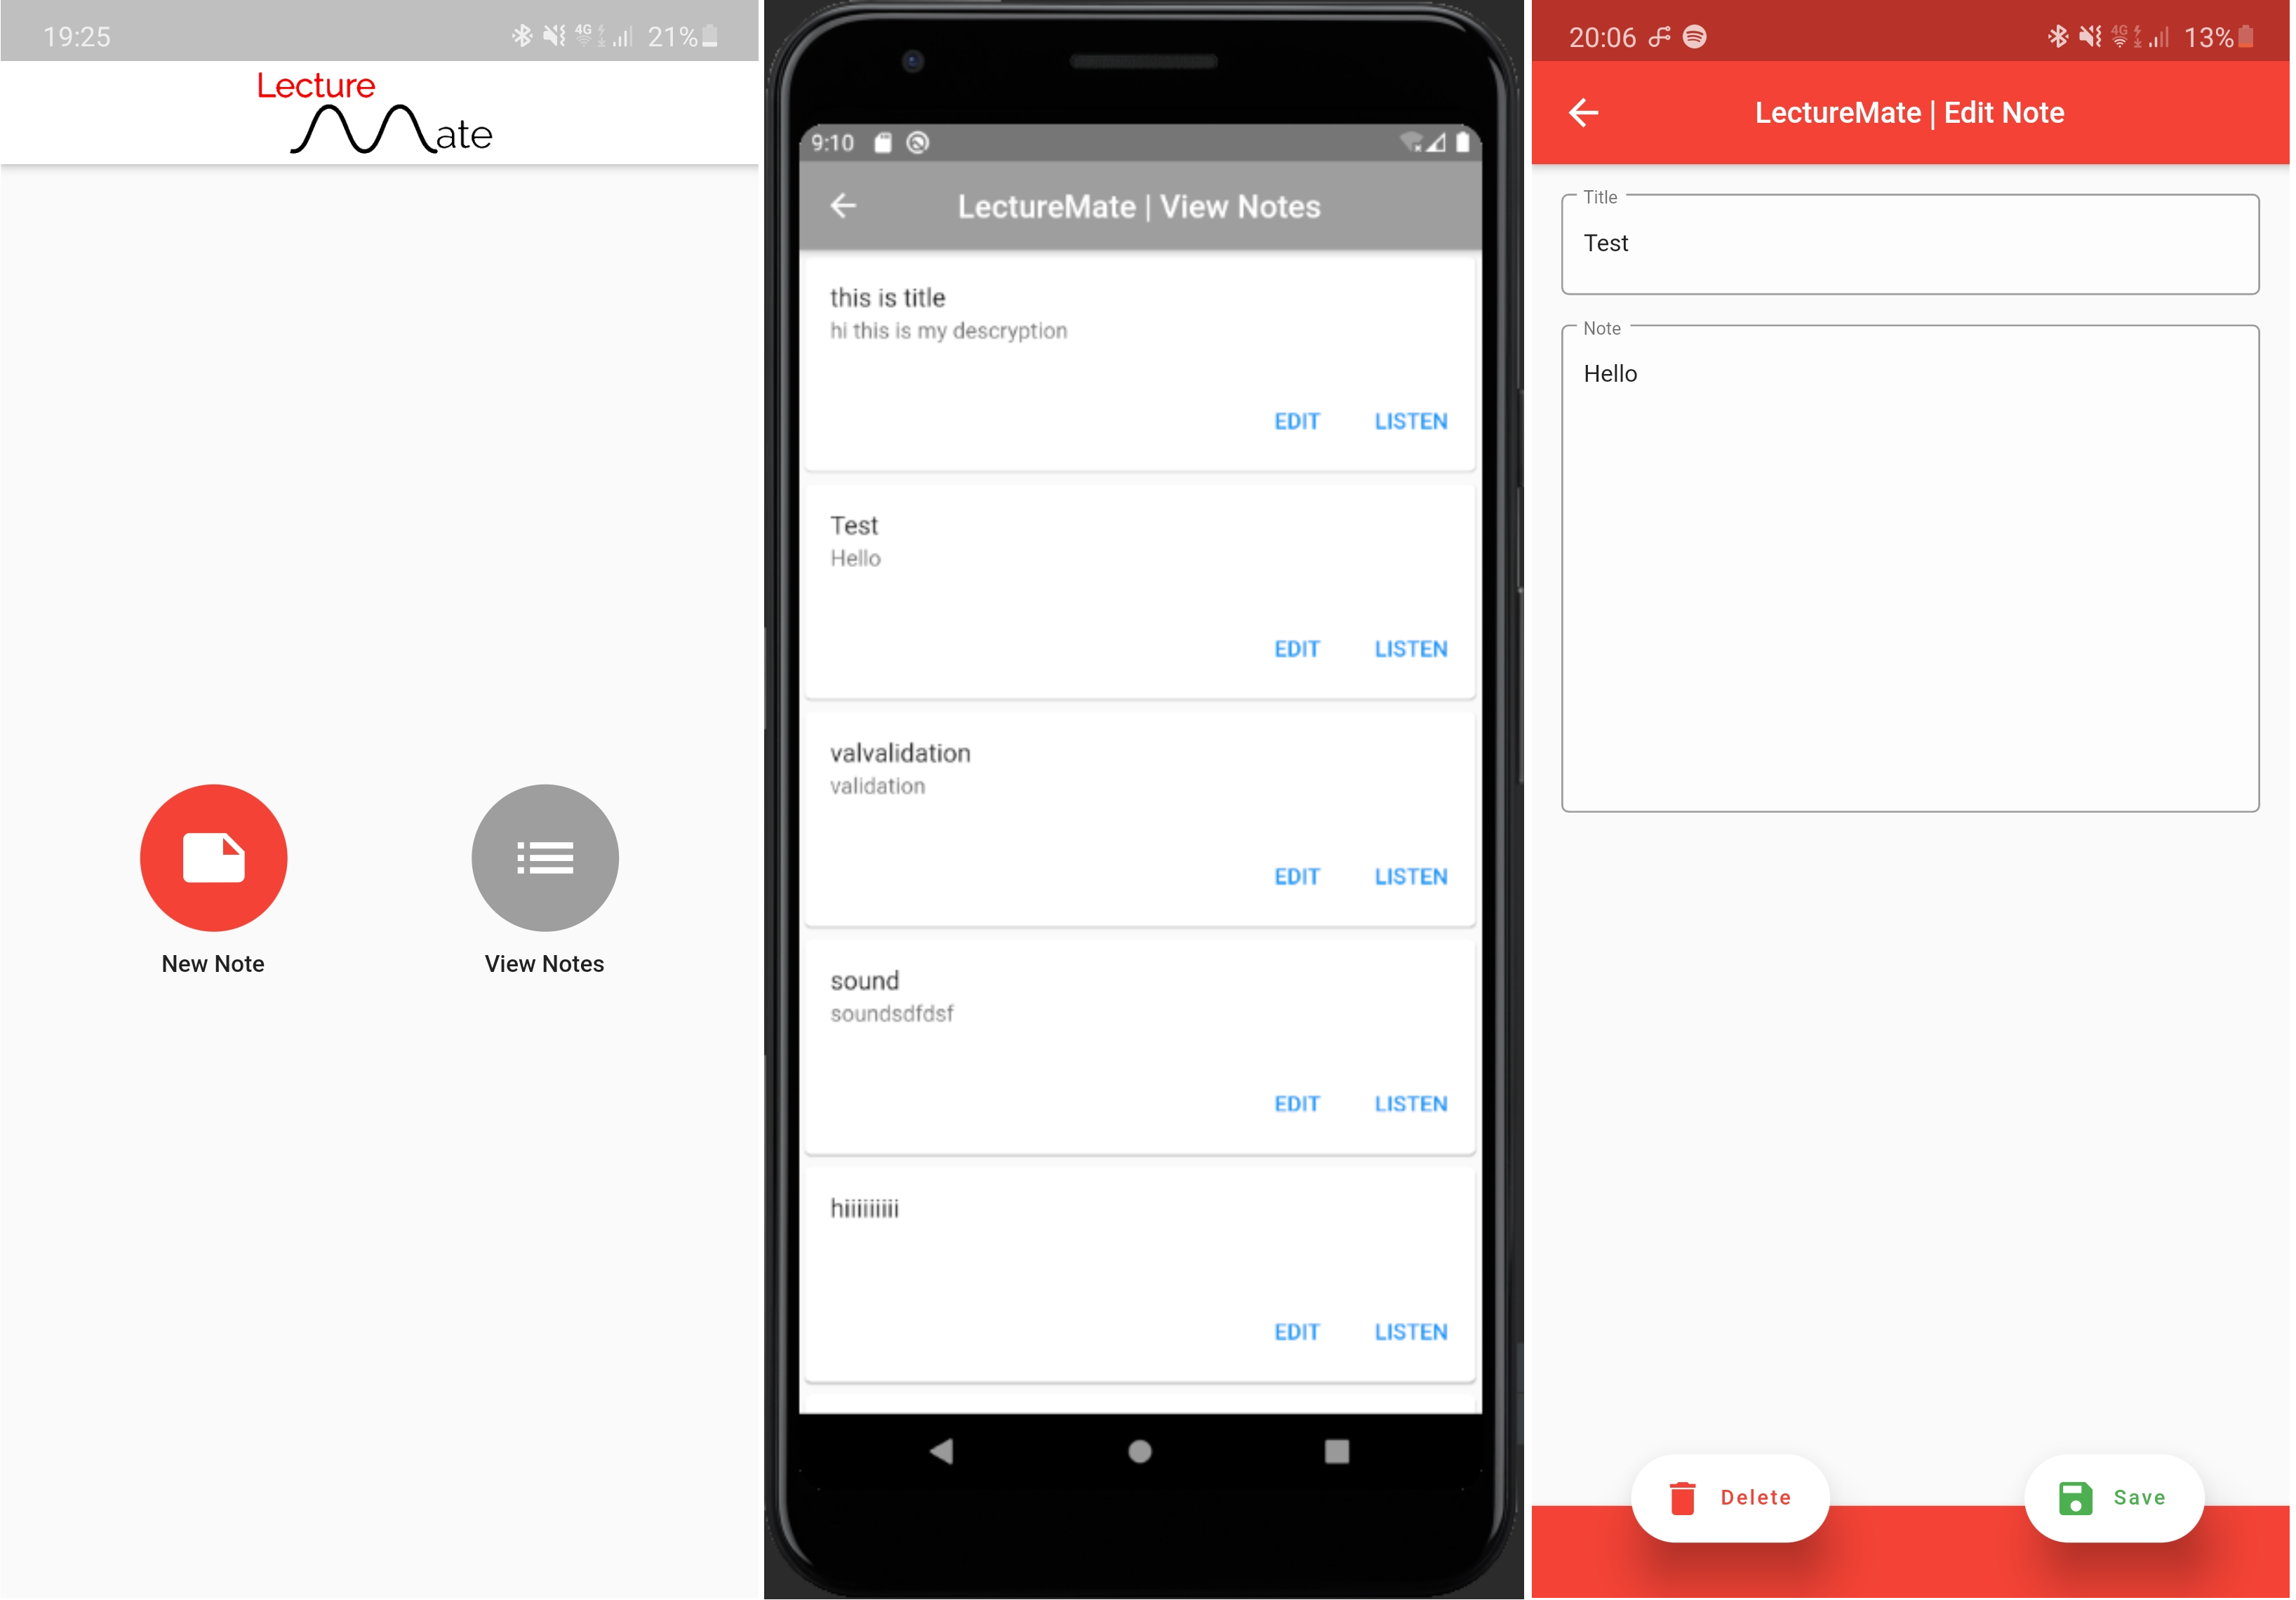
\includegraphics[width=6in]{/editnote_process.png}}
			\end{center}
			\caption[Editing Note Process]{Editing Note Process}
		\end{figure}



%-----------------------------------------------------------------------------------------------
%					SYSTEM DESIGN
%-----------------------------------------------------------------------------------------------
\chapter{System Design}
	\section{Design Models}
		\subsection{Activity Diagram}
		I planned out the activities using an activity diagram which shows the not only the user's process requests but the systems process requests also. This illustrates the workflow of the application between the user and the system. This can be seen in \textbf{Figure 9.1 in Appendix A}.

		\subsection{Sequence Diagram}
		The Sequence Diagram shows the process of the interactions between the two consumers in sequential order. This would include the browsing of the application, the communication of the two consumers and also the transactions of the two consumers. The sequence diagram can be seen in \textbf{Figure 9.2 in Appendix A} where there is a clear, simplified version of what has been expected of the web application in the form of a Minimum Viable Release/Product, or MVR/MVP.

	\newpage

	\section{Prototypes}
	Prior to commencement on working on the UI of the application, I looked at the prototypes I had created at two different stages to gather feedback on whether they would be user-friendly and if users found the UI design engaging to gauge whether I needed to make any changes 		

	\section{UI Design}
		\subsection{Create Note}
		Features of the New Note UI are the two text editing controllers containing the Title and Body of the note, as well as this, the Audio recording button which on press will begin recording and finally two buttons which cancel the note with a popup dialog for confirmation and a save button to save the data to the database.\\

This is very similar to the Edit Note UI, however, it does not display the audio recording feature as this only allows for updating and a recording cannot be updated as such, thus only the title and note body text controllers are modifiable.\\

		\begin{figure}[H]
			\begin{center}
	 		 	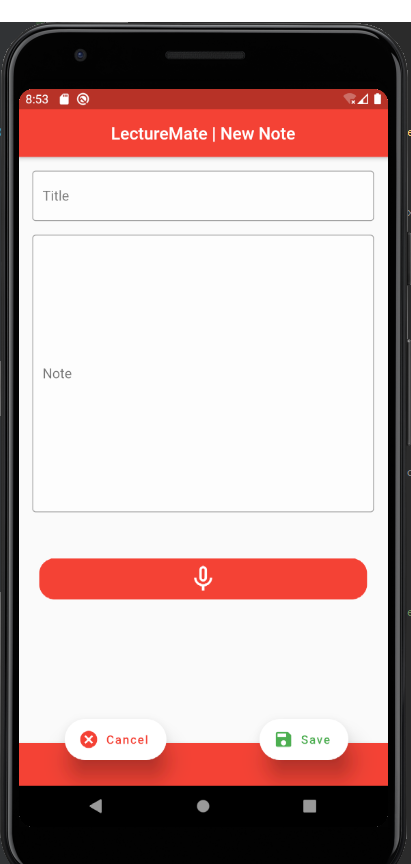
\includegraphics[width=2in]{/newnote.png}
			\end{center}
			\caption[New Note UI]{New Note UI}
		\end{figure}

%-----------------------------------------------------------------------------------------------

		\subsection{List Notes}
		The list notes UI is designed in such a way that it is clear, displaying each of the notes as cards which makes it easier to differentiate between them. The size of the cards are dependent on the content in the note, this consists of the title which is displayed above in a larger font proceeded by the note body in a smaller grey text.\\

The note card also has the option to edit the note where it navigates to the editNote page, referencing the note by it's unique ID, in the same way - any audio recording appended to the note can be listened to by pressing the 'Listen' button navigating to the playback screen.\\
		
		\begin{figure}[H]
			\begin{center}
	 		 	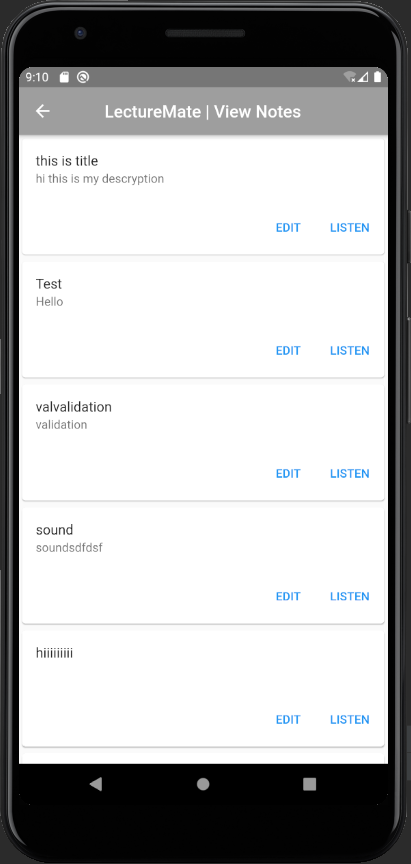
\includegraphics[width=2in]{/list.png}
			\end{center}
			\caption[List Notes UI]{List Notes UI}
		\end{figure}

%-----------------------------------------------------------------------------------------------

		\subsection{Recording}
		The recording UI is very simplistic, displaying the timer of the audio duration of the current position. As well as this, it gives the user two options - to either stop the recording, to which it will return to the New Note page appended to the note, awaiting submitting to the database.\\

Another option would be that the user can press the bookmark button, this action would take the current position of the audio recording and store this in a list as a bookmark which the user would be able to identify later on as an important section of the recording.

			\begin{figure}[H]
				\begin{center}
		 		 	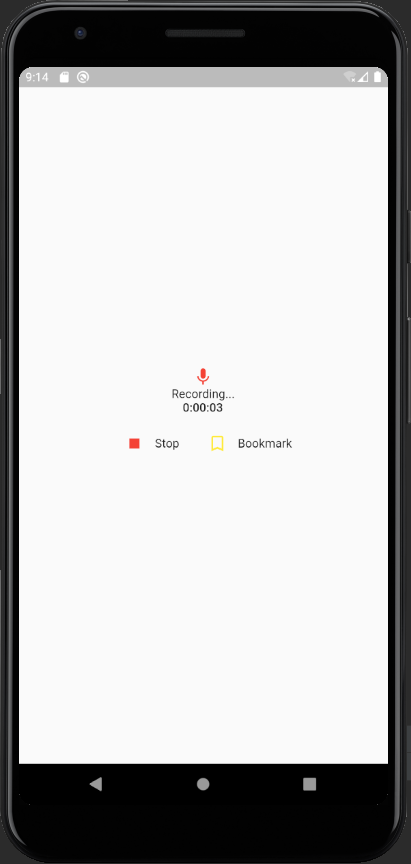
\includegraphics[width=2in]{/recording.png}
				\end{center}
				\caption[Recording UI]{Recording UI}
			\end{figure}

%-----------------------------------------------------------------------------------------------

		\subsection{Playback}
		Playback of the audio recording simply just plays and stops the recording. There is a single button in the centre of the frame whereby the icon changes state dependent on the state of the audio, i.e. when the audio is paused a play icon will display.\\

The playback control operations are carried out using a library which takes the audio file as an input and plays this aloud. Further features which are yet to be added is a seeking feature allowing the user to scroll within the recording.

			\begin{figure}[H]
				\begin{center}
		 		 	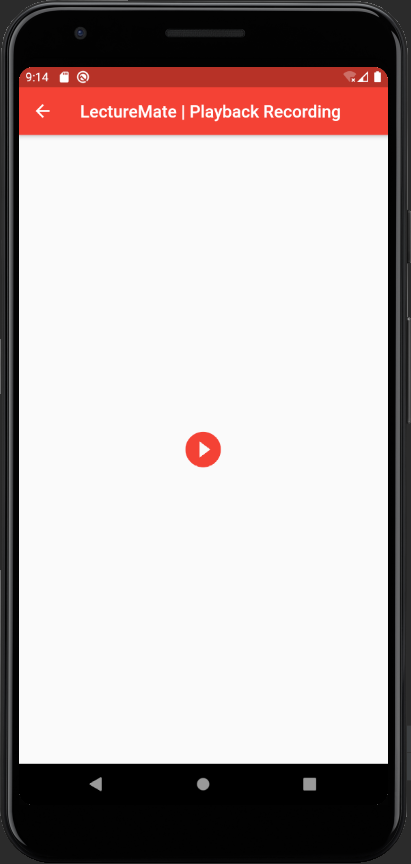
\includegraphics[width=2in]{/playback.png}
				\end{center}
				\caption[Playback UI]{Playback UI}
			\end{figure}

%-----------------------------------------------------------------------------------------------
%					IMPLEMENTATION
%-----------------------------------------------------------------------------------------------
\chapter{Implementation}
	\section{Front End - Flutter}
	 Front end web development, also known as "client side programming", is based on everything that happens in the user's interface. From the layout, user interface and user experience, it is what the users can see and interact with. Since the project heavily focuses on the user base, it was essential that existing and potential clients feel comfortable with using the application. I established early on in the project that a mobile application would be best as it is the most easily accessible via multiple range of smart phones.\\
	
	The front end was handled by the Flutter package which makes use of the Material package as part of Flutter. This managed the UI and layout of the application. Due to the nature and simplicity of use of this package, it was very easy to look at making the UI aesthetically pleasing and pretty from the time of implementation - whereas I was expecting to have to focus more on the functionality of the application and then later look at making the UI more user friendly.

	\section{Business Layer - Flutter}
	The business layer which is the layer which handles the communication between the front-end and back-end operations - this is also written using Flutter as it has the ability to seamlessly link both the Flutter framework and the Google Firebase database. \\
	
	This consists of the database.dart file which acts as a database helper file containing the functions to submit and retrieve the data to and from the database. As well as this, due to potential unreliable internet connections, offline use has been considered where the audio recording is stored locally in case it has not been possible to upload to the database. \\
	
	Apart from this the other business layer functions are execute in smaller sections within classes in the code which can be seen in more depth in the Code Review section which proceeds after this.

	\section{Back End - Google Firebase}
	The back-end is managed entirely by Google Firebase, which as a Google product works well with Flutter which is also developed by Google. It is controlled through script written using the database helper which contains functions to execute CRUD functions in the database.\\

The database is a NoSQL database which is made up of collections, in the case of this application, a single collection 'notes' which contains documents which is each note uploaded in the application. The format of each note is the Tite, Body of the note, the Audio Recording URL and Recording Duration.\\

When being retrieved from the database, the application takes the URL of the audio recording and plays this back using the playback feature to add better functionality and ease of use to the users.

	\section{Mobile Application Development}
	Using Flutter has allowed the development of the application to be written once using the Flutter engine and can be used on both Android and iOS devices with no compatability issues which may depend on the platform.\\

This is a huge advantage as it allows the application to be deployed to users of both these devices and it can grow rapidly with continuous integration in potential developments in later revisions of the application. \\

The development and implementation phase was spread over a long period of four to five months whereby I was able to tackle each feature and spend a reasonable amount of time making sure that they would work as expected. Initally, I decided to focus on the functionality over the appearance and UI of the application. However, the ease of use of Flutter allowed the appearance to be worked on easily in a short space of time which working on the functionality. \\

I would utilise Version Control in the form of Git to manage the code and see the changes I had made to keep track of the progress made as well as have a backup in case of loss of work or to rollback changes which had caused major or significant issues to the application. This was very helpful as it  also meant I could review my code and spend time looking at whether any code was redundant or could be made redundant to simplify the code for clarity and speed when compiling the application at each stage.

	\section{Code Review}
	I reviewed the code I have for the application to explain the workings and how they contribute to the functionality. I will analyse and review each of the most important classes in the code to give a brief but clear understanding of their implementation:

		\subsection{database.dart}
		As previously mentioned, I have included a database helper file to manage the CRUD operation and functions between the front end application and Firebase database.\\

The way in which it works is firstly by using the packages to access the Firebase Storage (Firestore) and Database as well as packages used to store the timestamp of the notes (Intl) and to upload files (Dart.io).\\

Firstly, a new collection reference is crerated where the collection in the database, notes, is referred to and this is initalised so that all functions will access this to execute the operations:

			\subsubsection{uploadingNote}
			A condition is set to check whether a voice\_note has been added to the note, if not, the title, body and timestamp of the note are uploaded to the database. If an audio recording has been added, this is uploaded to Firebase Storage (Firestore) and the unique id is stored and is called in the upload of the note alongside the other parameters where the audio file URL will also be stored. 

			\subsubsection{getNotes}
			A List data structure is created to retrieve the list of notes in the database, referred to as a Snapshot. This reference is then used to get all the documents saved in the database, a for statement is then used to itemise each of the notes by the total there are stored and these are returned.

			\subsubsection{editNote}
			The notes collection is referenced and the document to be updated is retrieved using the document ID and this obtains the title and body of the note and in the editNote class this is displayed in the Text Editing Controllers to allow the user to make changes to the note.

			\subsubsection{deleteNote}
			This function simply deletes the note upon the users decision. Similar to the editNote function, it is referred to by its Document ID and then this is deleted.

		\subsection{newNote.dart}
The main function within the newNote.dart is the submit function, which initially sets the state of the uploading boolean to true preparing the database to receive data. The Database function is called from the database helper class, database.dart which takes the parameters of the note to be uploaded.\\

The database makes use of the async operation which asynchronously uploads the data to the database and listen for a result from the database.\\

These parameters include the title of the note, the body text and if recorded, any audio recordings which are processed by the Database function and submitted to the database. Finally, the state of the recording boolean is reset to false and the recording is cleared and the screen returns to the main homepage.
		\begin{figure}[H]
			\begin{center}
	 		 	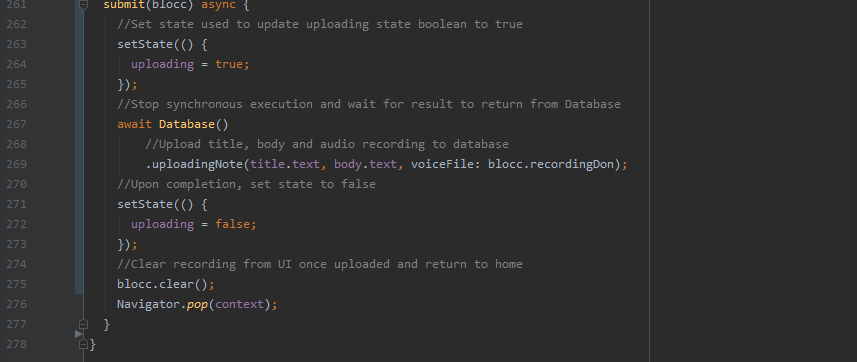
\includegraphics[width=6in]{/newnote_code.png}
			\end{center}
			\caption[New Note]{New Note}
		\end{figure}

%---------------------------------------------------------------------------------------------------

		\subsection{list.dart}
		The list class works by essentially retrieving the data from the database and displaying these as a list.\\

More specifically, a List data structure is created called, Notes, which contains an empty array. Then the database helper is accessed and the function getNotes() is executed with the return prompting a condition which sets the notes to take the notes stored in the database into the array.\\

This is then followed by the updateList() function which carries out the same function but updating the list with any new additions of notes - this function will generally be executed when the list page is accessed.
		\begin{figure}[H]
			\begin{center}
	 		 	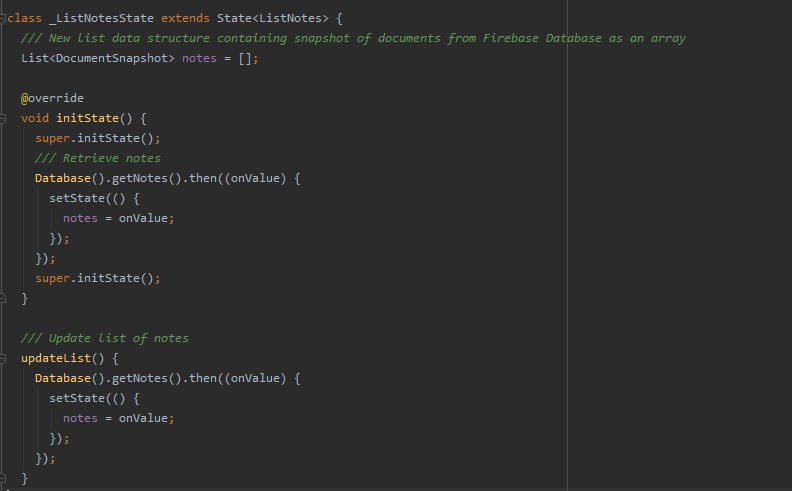
\includegraphics[width=6in]{/list_code.png}
			\end{center}
			\caption[View Notes]{View Notes}
		\end{figure}

%---------------------------------------------------------------------------------------------------

		\subsection{playback.dart}
		The playback of the audio files are very simple and make use of the built-in AudioPlayer function from the flutter-audio-player package. \\

First of all, an instance of the audioPlayer is created as well as some variables to monitor the playback of the audio, these include a boolean monitoring whether or not the audio is playing (\_isPlaying) which is initially set to false as nothing will be playing upon commencing the playback window. As well as this, there is the duration of the audio file assessing whether the file has reached the end of its max duration and can also be used with further developments, namely seeking in the audio file.\\

Finally, it also contains a dispose function, which as it is self-explanitory, disposes of the audio from the player on the stop button press. Part of this, allows for the audio to be played in the background while returning to the note when editing. 

		\begin{figure}[H]
			\begin{center}
	 		 	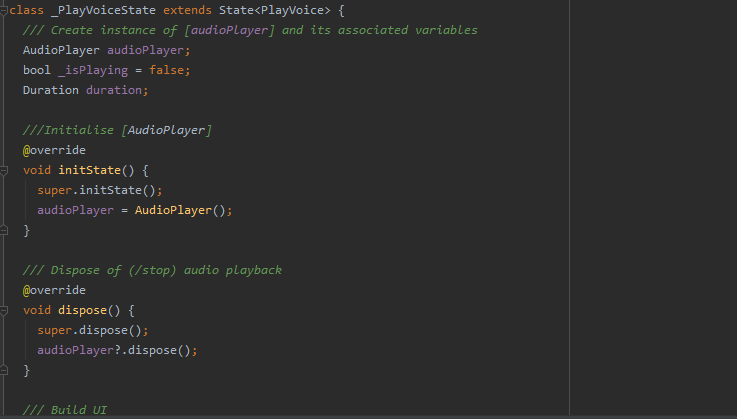
\includegraphics[width=5in]{/playback_code.png}
			\end{center}
			\caption[Recording Playback]{Recording Playback}
		\end{figure}

%---------------------------------------------------------------------------------------------------

		\subsection{voice\_message.dart}
		Voice message contains many functions which contribute to the operation of this feature - these consist of \_prepare, \_startRecording, \_stopRecording, and \_init functions:

		 \begin{enumerate}
		 	\item \_prepare gets the recorder ready to record obtaining all the prerequistes needed. This being making sure the application has the correct permissions enabled for the recording to begin, this being permissions to allow the application access to the microphone as well as to the device files to save the recording locally once complete.\\

If the permissions are enabled, the recorder is ready awaiting the command to start recording.
			\item \_startRecording function simply awaits for the recorder to start, this is executed when the button as part of the UI side is pressed on which can be seen in \textbf{Figure 5.1}\\

The recorder state is then set to current as it begins recording and a timer is begun in order to track the duration elapsed since the recording had began and this valie is returned to the UI, this continues until the recorder has stopped.
	
		  	\item \_stopRecording occurs when the Stop button has been pressed from the UI which sets the state of the recording to result which stops the timer and returns the audio name and duration to the UI displayed below the text body box. Lastly, the \_checkForStop boolean is set to false as the recorder has since been stopped.\\

			\item \_init is where the function for storing the audio file is executed whereby the path of where this is saved is defined in the directory of the device. This contains the name of the audio file which is made up from the date and timestamp it was recorded and the file extension which is hardcoded but can be changed to fit other file types.\\

However, this file type was chosen as the application was designed for use on both Apple and Android devices and these devices both support the encoding of these file types ensuring greater accessibility of the application.
		 \end{enumerate}

		\begin{figure}[H]
			\begin{center}
	 		 	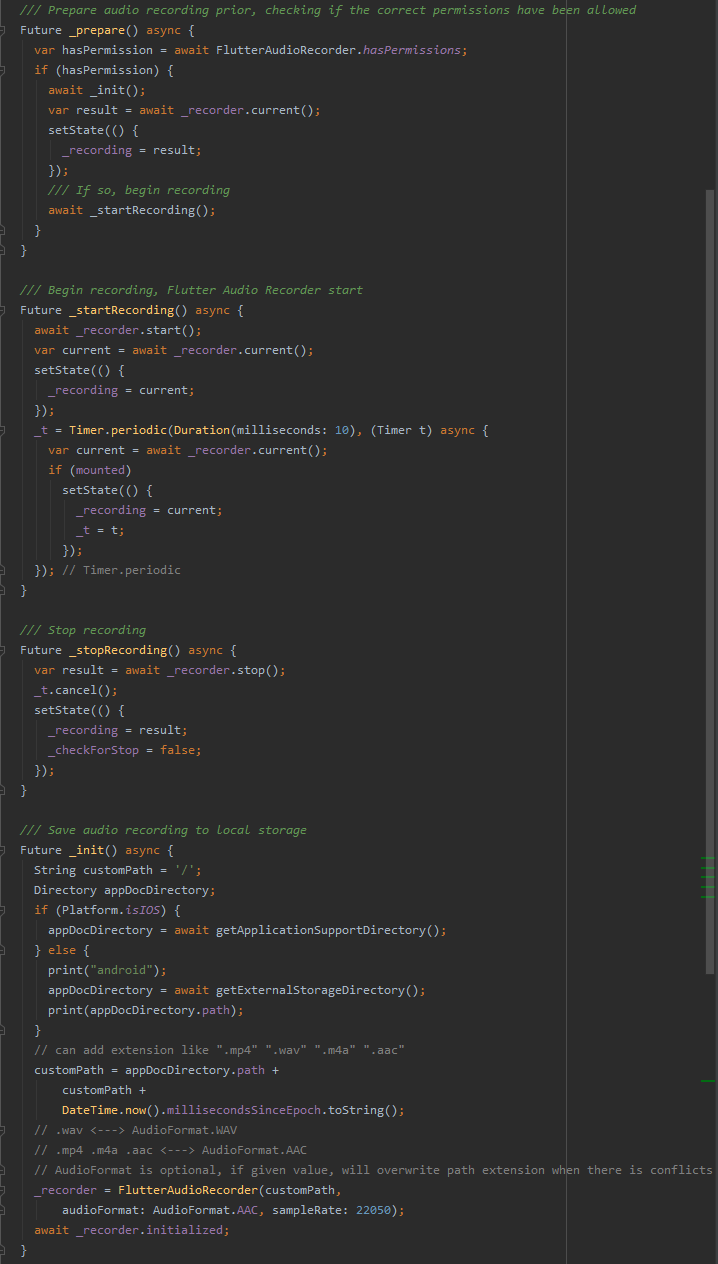
\includegraphics[width=3.75in]{/recording_code.png}
			\end{center}
			\caption[Record]{Record}
		\end{figure}

%---------------------------------------------------------------------------------------------------

	\section{Disruptions and Solutions}
		 \begin{enumerate}
			\item Bug 1: As can be seen in \textbf{Figure 9.2 of Appendix B}, one of the issues I had with the code was regarding the Front-End where the Scaffold which is part of the Flutter package managing the structure of the User Interface of the application has issues. the issue being that the type in which I was trying to define a new component as part of the scaffold was not that of what it needed to be producing the error as per the figure.\\

The way in which I went about resolving this was in three stages, where initially, I combed through the code to see where the error might lie as a particular line number was not referenced as to throwing error and failing to find the error, I research online to see whether this was an error which others may have faced and provided a suitable solution to which there was which was to use another structure within the scaffold which would achieve the same result. Finally, I went about trial and error to see where the issue was found until I was able to locate and implement the change to provide a good solution.

		 	\item Bug 2: As can be seen in \textbf{Figure 9.3 of Appendix B}, the second bug I faced was to the List feature of the application which maintains the purpose of updating itself with the notes which are stored on the database.\\

It makes use of a class called a Document Snapshot which runs a query on the collection of the notes which should then be returned to the View Notes UI for the user to review and make changes to.\\

The error I was having was in printing the returned results of the Document Snapshot directly into new elements of an array. However, it was not able to handle the response as it would not print each note to a new element in the array but force multiple results into a single element which caused the exception.\\

The way in which I resolved this was by following a similar process to the prior bug in going through the code to find and isolate the individual part of the code this was affecting and later find a solution. After I was able to identify this, I carried out research to find solutions to this problem to which I came across using a List data structure to hold the Document Snapshot query and then return each result of this query using a for statement of each result to print to a new element in the array. This was able to solve the issue instantly and caused no further problems and later changes to take an additional parameter of the audio recording URL.
		 \end{enumerate}
		 
	\section{Deployment}
	Software deployment is the activities which make the application available for use. The application essentially is ready for use and can be progressed to the deployment stage. As it is, it satisfies the MVP with all the integral features. \\

As mentioned before, there is the scope to add additional features to improve the look and functionality of the app and so deployment would use the CI/CD (Continuous Integration/Continuous Deployment) and release each feature in revisions of the app and testing would be done prior to every release to ensure that additional features have not adversely affected the current features from the previous release. \\

As the application has been developed following the agile methodology it makes better sense to use CI/CD as it allows for better focus on reliability, code quality and security of the application due to the fact that the deployment steps are automated. \\

Upon each stage of a new release, updated documentation and guides will be provided for better understanding of the changes as well as any bugs which were reported after initial deployment and whether these have been resolved.\\

The process in deploying the application would be as follows:

\begin{itemize}
	\item Ensure the application works with no obvious, visible bugs.
	\item Check that the application has satisfied the requirements and met the MVP.
	\item Demonstrate and gather feedback and approval from the end users.
	\item Produce documentation to ensure the application is usable and clear for the end user with the documents there to provide any support.
	\item Release and deploy the application upon approval.
\end{itemize}

%-----------------------------------------------------------------------------------------------
%					TESTING
%-----------------------------------------------------------------------------------------------
\chapter{Testing}
	\section{Testing Criteria}
	Prior to conducting the testing, the criteria had to be set out in order to have guidelines to what the testing would need to achieve in order for the function to be classed as working correctly. 
	
		\subsection{A/B Testing}
		A/B testing looks at the prototypes at the beginning of the project to obtain feedback on whether this system satisfies the users need and essentially to  build a specification for the application. Two prototypes were created and at both stages, testing and feedback was obtained on whether they met the aim of the tests.\\
		
Feedback received from potential end users were that the application was clear, user-friendly and had great potential - this being at the first Paper Prototype. Moving forward, taking this feedback into consideration, the high-fidelity prototype was created to make a more interactive and give the users more of a feel to the look of the final application. This brought great feedback and the users stated that the application looks very professional and something they would use regularly, discarding their current methods of taking notes.
	
		\subsection{White and Black Box Testing}
		
		The features would be tested using the Black Box and White Box test method. Black box testing looks at whether the feature works as expected against the expected output. White box testing however, looks at whether the function in the code returns the correct output. These methods are displayed in \textbf{Table 7.1} below.\\
		
		The following table detail test cases that are assessing the overall application. Some of the test cases produced are repetitive but that is to ensure everything is working and is fairly tested:
		
		\begin{table}[H]
		\centering
		\caption{Testing Criteria}
		\begin{tabular}{|l|l|l|l|} 
		\hline
		Test \# & Test Type & Description & \begin{tabular}[c]{@{}l@{}}Expected\\Outcome\end{tabular} \\ 
		\hline
		1 & \begin{tabular}[c]{@{}l@{}}Black\\Box\end{tabular} & \begin{tabular}[c]{@{}l@{}}Click App Icon from\\App Drawer\end{tabular} & Opens Splash Page and loads to Home Page \\ 
		\hline
		2 & \begin{tabular}[c]{@{}l@{}}Black\\Box\end{tabular} & \begin{tabular}[c]{@{}l@{}}New Note \\Button Press\end{tabular} & Opens to Blank New Note Page \\ 
		\hline
		3 & \begin{tabular}[c]{@{}l@{}}Black\\Box\end{tabular} & \begin{tabular}[c]{@{}l@{}}Edit Note \\Button Press\end{tabular} & Opens to List Page, listing all notes \\ 
		\hline
		4 & \begin{tabular}[c]{@{}l@{}}Black\\Box\end{tabular} & \begin{tabular}[c]{@{}l@{}}Cancel Dialog -~\\New Note\end{tabular} & \begin{tabular}[c]{@{}l@{}}Cancel dialog - (Yes) Return to Home Screen,\\(No) Return to current note\end{tabular} \\ 
		\hline
		5 & \begin{tabular}[c]{@{}l@{}}Black\\Box\end{tabular} & \begin{tabular}[c]{@{}l@{}}Delete Dialog -~\\Edit Note\end{tabular} & \begin{tabular}[c]{@{}l@{}}Delete dialog - (Yes) delete note, \\(No), return to note\end{tabular} \\ 
		\hline
		6 & \begin{tabular}[c]{@{}l@{}}Black\\Box\end{tabular} & \begin{tabular}[c]{@{}l@{}}Submit Blank Note -~\\New Note\end{tabular} & Validation check prompt \\ 
		\hline
		7 & \begin{tabular}[c]{@{}l@{}}Black\\Box\end{tabular} & \begin{tabular}[c]{@{}l@{}}Record button - \\New Note\end{tabular} & Automatically begin recording~ \\ 
		\hline
		8 & \begin{tabular}[c]{@{}l@{}}Black\\Box\end{tabular} & \begin{tabular}[c]{@{}l@{}}Stop -\\Recording\end{tabular} & \begin{tabular}[c]{@{}l@{}}Recording Stops - Returns to New Note Page\\displaying the Recording and Duration\end{tabular} \\ 
		\hline
		9 & \begin{tabular}[c]{@{}l@{}}Black\\Box\end{tabular} & \begin{tabular}[c]{@{}l@{}}Bookmark -~\\Recording\end{tabular} & \begin{tabular}[c]{@{}l@{}}Bookmark current position in recording and~\\show this as a list in the New Note Page\end{tabular} \\ 
		\hline
		10 & \begin{tabular}[c]{@{}l@{}}Black\\Box\end{tabular} & \begin{tabular}[c]{@{}l@{}}Play Icon -~\\Playback\end{tabular} & \begin{tabular}[c]{@{}l@{}}Playback should begin of the audio recording\\of the corresponding note\end{tabular} \\ 
		\hline
		11 & \begin{tabular}[c]{@{}l@{}}Black\\Box\end{tabular} & \begin{tabular}[c]{@{}l@{}}Stop Icon -~\\Playback\end{tabular} & \begin{tabular}[c]{@{}l@{}}Playback should stop of the audio recording~\\of corresponding note\end{tabular} \\ 
		\hline
		12~ & \begin{tabular}[c]{@{}l@{}}Black\\Box\end{tabular} & Save - New Note & \begin{tabular}[c]{@{}l@{}}Note should be saved to the database containing\\Title, Body and Audio\end{tabular} \\ 
		\hline
		13 & \begin{tabular}[c]{@{}l@{}}Black\\Box\end{tabular} & Save - Edit Note & Overwrite existing note and save to database \\ 
		\hline
		14 & \begin{tabular}[c]{@{}l@{}}Black\\Box\end{tabular} & Edit - View Notes & \begin{tabular}[c]{@{}l@{}}Note should load with text fields populated with\\corresponding note from the database\end{tabular} \\ 
		\hline
		15~ & \begin{tabular}[c]{@{}l@{}}Black\\Box\end{tabular} & Listen - View Notes & \begin{tabular}[c]{@{}l@{}}Playback should open of audio for corresponding\\note from the database\end{tabular} \\ 
		\hline
		\multicolumn{4}{|l|}{} \\ 
		\hline
		16 & \begin{tabular}[c]{@{}l@{}}White\\Box\end{tabular} & uploadingNote() & \begin{tabular}[c]{@{}l@{}}C - Upload all parameters (title, body and audio\\recording to Firebase Database\end{tabular} \\ 
		\hline
		17 & \begin{tabular}[c]{@{}l@{}}White\\Box\end{tabular} & getNotes() & R - Retrieve all notes stored on Firebase Database \\ 
		\hline
		18 & \begin{tabular}[c]{@{}l@{}}White\\Box\end{tabular} & editNote() & \begin{tabular}[c]{@{}l@{}}U - Update note in database overwriting exisiting\\data\end{tabular} \\ 
		\hline
		19 & \begin{tabular}[c]{@{}l@{}}White\\Box\end{tabular} & deleteNote() & D - Delete note from database \\
		\hline
		\end{tabular}
		\end{table}
			
		\subsection{Stress and Performance Testing}
		Stress and Performance testing is used to gather whether the application is able to handle the processes within the application, ensuring stability, reliability and usability. It is monitored by the speed at which it returns the expected result and whether it returns the correct result. The results of this test can be seen in \textbf{Table 7.2.2}.
		
		\subsection{Beta Testing}
		Beta testing is the process of testing the system prior to release among a group of potential end users to obtain feedback of whether the MVP has been met and it ready for release. This stage also allows us to identify any remaining bugs which can be resolved prior to deployment - this being so it is produced at the highest standard at this inital stage.The results of this test can be seen in \textbf{Table 7.2.3}.

	\section{Testing Results}
	This was the result of the test cases that showed whether it was a success when conducting different features of the mobile application.\\

		\subsection{Black and White Box Testing}
		
		The following Table (\textbf{Table 7.2}), lists the outcome of the results for Black and White Box testing:
		
		\begin{table}[H]
		\centering
		\caption{Testing Criteria}
		\begin{tabular}{|l|l|} 
		\hline
		Test \# & Pass/Fail? \\ 
		\hline
		1 & Pass \\ 
		\hline
		2 & Pass \\ 
		\hline
		3 & Pass \\ 
		\hline
		4 & Pass \\ 
		\hline
		5 & Pass \\ 
		\hline
		6 & Pass \\ 
		\hline
		7 & Pass \\ 
		\hline
		8 & Pass \\ 
		\hline
		9 & Pass \\ 
		\hline
		10 & Pass \\ 
		\hline
		11 & Pass \\ 
		\hline
		12~ & Pass \\ 
		\hline
		13 & Pass \\ 
		\hline
		14 & Pass \\ 
		\hline
		15~ & Pass \\ 
		\hline
		\multicolumn{2}{|l|}{} \\ 
		\hline
		16 & Pass \\ 
		\hline
		17 & Pass \\ 
		\hline
		18 & Pass \\ 
		\hline
		19 & Pass \\
		\hline
		\end{tabular}
		\end{table}
		
		\subsection{Stress and Performance Testing}
			\begin{table}[H]
			\centering
			\resizebox{\textwidth}{!}{%
			\begin{tabular}{|l|l|l|l|l|}
			\hline
			Type & Description & \begin{tabular}[c]{@{}l@{}}Expected\\ Outcome\end{tabular} & \begin{tabular}[c]{@{}l@{}}Actual\\ Outcome\end{tabular} & Result \\ \hline
			\begin{tabular}[c]{@{}l@{}}Stress \&\\ Performance\end{tabular} & Loading time & \begin{tabular}[c]{@{}l@{}}The application should load to \\ the main page within 5 seconds\end{tabular} & \begin{tabular}[c]{@{}l@{}}The application loaded to \\ home screen in 3 seconds\end{tabular} & Pass \\ \hline
			\end{tabular}%
			}
			\caption{Stress and Performance Testing}
			\label{Stress and Performance}
			\end{table}
			
		\subsection{Beta Testing}
			\begin{table}[H]
			\centering
			\resizebox{\textwidth}{!}{%
			\begin{tabular}{|l|l|l|l|l|}
			\hline
			Type & Description & \begin{tabular}[c]{@{}l@{}}Expected\\ Outcome\end{tabular} & \begin{tabular}[c]{@{}l@{}}Actual\\ Outcome\end{tabular} & Result \\ \hline
			Beta & User testing & \begin{tabular}[c]{@{}l@{}}The application should run\\ without bugs and to users satisfaction\end{tabular} & \begin{tabular}[c]{@{}l@{}}No bugs, users satisfied with appearance \\ and functionality.\end{tabular} & Pass \\ \hline
			\end{tabular}%
			}
			\caption{Beta Testing}
			\label{Beta}
			\end{table}

	\section{Formative Evalutation}
	Following the Agile development method, I followed the cycle of implementing changes and testing at each phase and repeated this until the MVP was met. This helped me to ensure that each of the requirements defined were met and that I would satify the inital requirements set by user feedback at the research stage. \\
	
This preparation allowed me to focus on the implementation and not have to worry about which features to implement at the next phase which meant I was more efficient and little to no time was wasted. As a result, when it came to the testing stage, because I prepared well and executed this correctly, it meant I was able to pass the tests without fail acheiving the MVP.\\

The features at the time of specification had all been agreed and confirmed with my supervisor so that I knew I would be able to develop an application with enough complexity at the MVP stage and passing these meant I had satisfied it.

	\section{Functional Requirements Evaluation}
	To be able to meet the requirements of the applications. Testing of the application was done in order to ensure the usability of the mobile application. These testing criteria are the main functionality was deemed from the \textbf{Table 4.1}. The testing for the application was done which can be seen in \textbf{Section 7.1}. The following is the evaluation of the functionality of the application.\\

	\begin{itemize}
		\item FR01 - The application makes use of the Flutter framework allowing it not to be limited to one device but any Android device which it is able to do upon testing on an Emulator and physical device.
		\item FR02 - The application requires constant access to a relaible internet connection due to the fact that the app relies heavily on the Google Firebase database where all data is stored, this meaning that any data input while there is an internet connection will be successfully submitted and stored to the database for later access.
		\item FR03 - The application saves notes to the Google Firebase database, however, these are not authenticated in any way and so allows any user who has access to the application can add or modify notes. This is secure in the sense that if the application is shared amongst a selective group then it can remain secure. The application is developed in such a way that only those who have access via a token to the database can access it.
		\item FR04 - The application has the facility to store the recordings to local storage on the device and upon the end of the voice recording, the audio file is uploaded to Firebase Storage and referenced to Firebase Database.
		\item FR05 - Some of the main features part of the application are to make notes and be able to review these notes which the application does allow them to do.
		\item FR06 - The application makes use of Google Firebase, which allows for the CRUD operations when using the application, this is best illustrated in the testing criteria where in the White Box testing the CRUD functionality of each of the operations demonstrates that these are implemented successfully in the application.
	\end{itemize}

	\section{Non-functional Requirements Evaluation}
	This is checking if the non-functional requirements have been met which is detailed in \textbf{Section 4.1.2}. These are explaining the standards the mobile application must satisfy.

	\begin{itemize}
		\item NFR01 - The mobile application is developed using the Flutter framework using the Dart language, this has ensured that the application can be used on both iOS and Android devices, however, testing has only been completed on an Android Emulator as well as a physical Android device to which the app works as expected on.
		\item NFR02 - User testing would be able to satisfy this requirement as it uses assumes that the person has not used the application before and would be able to test whether they are able to carry out all the functions without any errors and all behaviours are as expected.
		\item NFR03 - The data is stored in the Google Firebase database which in itself is secure as it only allows anyone with a token to access it. However, if deployed and the application is shared, unauthorised users can maliciously edit and delete notes from the database.
		\item NFR04 - The application in its current form does not have any visible bugs and works as expected passing all testing criteria in the black and white box testing methods. However, subject to other testing methods such as Performance and Stress Testing may provide some other bugs which have not appeared as yet.
		\item NFR05 - The application loads within 3 seconds on opening and all operations are executed well within the 10 second ideal criteria. However, this has been tested only with a reliable internet connection - testing with a slower, or more unreliable internet connection may produce different results but in this case it meets the requirement well.
	\end{itemize}


%-----------------------------------------------------------------------------------------------
%					CONCLUSION
%-----------------------------------------------------------------------------------------------
\chapter{Conclusion}
	\section{Summative Evaluation}
		The overall objective of this project was to create a new approach for the issues in note taking applications in the targeted educational and academic environment. However, the application will not be limited to this scope. The aim of the application of to solve the issue of having useful features from several apps all in one space which allows for better cohesion and clarity in notes, especially in reviewing and/or revision. \\

The objective therefore, is to create a single space which enables the user to have all these features in one app. These features include making notes, adding attachments such as pictures, video or files such as PDFs or presentations but the main feature which the notes would be centered around would be the audio recording. Initially, I had thought to focus on working on the back end and making sure the functionality of the application would work before looking at the user interface and front end side of things.\\

The functionality of the backend was heavily reliant on the database and so the CRUD (Create, Read, Update and Delete) operations were made sure to be working for the rest of the application to function. Making use of Google Firebase to use as storage of data allowed for easier access due to the automatic generation of code to link the database to the application as Google had already done this. \\

Using Flutter enabled the use of packages whereby I was able to connect to the database and use existing functions to execute the operations needed. After working on the back-end, I moved onto the front-end to look at structuring the user interface which is the users view of the application. The front-end was built entirely using the dart language utilising the Flutter framework which uses a structure called a Scaffold which nests each component within the a layer. \\

The front-end has simple components all of which carry out the required functions. These consist of buttons and text boxes only with cards which display the notes as a list.\\

The middleware in this application was perhaps the most important layer as it manages the processes between the user interface and database. The middleware uses Flutter whereby the packages for the database access are used and the the functions will be executed. \\

I found the middleware most difficult in implementing as it contained the functions to carry out the CRUD operations. More specifically, the feature which was most difficult to implement was the creation of a note when appending the audio file to the note. I managed to implement the audio recording and was able to store this locally once complete which I had as a specification to meet the MVP. The issue I had was then uploading the audio file to the database as it is not raw data to be able to upload. \\

Therefore, I had to store the audio file to the Firebase storage and then reference the file in the storage as a URL to be accessed by the database which the application is able to read and then play this through the playback feature taking the URL as the input.\\

I had to research this as there were a few methods to complete this function but it was a case of which would be more efficient and effective. I could convert the audio file to a byte raw data to be stored in the database and read from the application and converted back to a file to be played but this would not be viable. \\

The option I went with was as previously mentioned to store this in the Firebase storage and reference it to playback audio. Using the built in functions of the library, queries did not have to be written to perform CRUD functions but were put through a function to take these as an input and output the result a a return. The biggest challenge faced in implementation was learning how to use flutter to build the application. Additional research and practice had to be done to learn to overcome any issues. I had to go about this through trial and error making sure I was able to ensure functionality. \\

Due to the current pandemic situation (Covid-19) it was more difficult to develop the app to a higher standard due to the lack of contact I was able to have to meet with the potential target to gather feedback and so I had to go based on feedback I had already received at the prototype stage. Therefore, I had to work on perfecting the application in terms of its functionality making sure there were no bugs and it would be suitable in appearance and essentially ready for deployment. 

	\section{Potential Future Development}
	The application allows major scope for future development and has the capacity to fulfil these, however, the main focus was to meet the MVP although these additional features can be seen in \textbf{Figure 9.1 of Appendix A} - some of these include, but are not limited to:

	\begin{itemize}
		\item User Settings: The user settings may contain the option for the user to enter a custom path to save the audio files locally, or not to store these locally at all. They may also include the registration and login at a later stage to control user permissions for use of the app at a later stage.
		\item Add Attachments: This was a feature which was conceived during the ideation of the application but was not a feature which is imperative to the application working and is likely to be a useful addition as users will have the ability to link or upload relevant files or media to the note which when it comes to review the note for revision purposes provides a more detailed and useful solution.
		\item Audio Waveform: The audio waveform is more of an aesthetic feature to look more appealing to users as they are able to see the waveform as the recording is going on. The waveform would be a precursor to other potential features.
		\item Highlight Bookmarks: The application when the recording is being executed has the option of bookmark which should create a list of all the important sections in the recording for review purposes so when seeking.
		\item Highlight Waveform Overlay: The overlay would use the bookmark points of the audio recording and have a visual feature which would show the user the most important sections of the audio which can be listened back to.
		\item Background Playback: This feature would allow the audio to be played in the background and perhaps when the device is locked. This feature would allow the user to make notes simultaneously to when notes are being made which is more useful than making notes after the recording is complete.
		\item Playback Control from Notification Bar/Lock Screen: Playback control from the notification bar or lock screen simply allows for more convenience for the user to control the audio when listening back.
		\item Playback Seeking: Playback seeking will allow the user to seek through the audio using the position in the recording and this will be useful with the highlights as you can seek to these important sections.
		\item Search Tool: A search tool will allow users to search for a note using a specific keyword which will display relevant results in the list page.
		\item Sort Tool: The sort tool allows the user to sort based on certain criteria, these might be based on alphabetical order or by date which the user might find useful.
	\end{itemize}
	
%----------------------------------------------------------------------------------------
%					 BIBLIOGRAPHY
%----------------------------------------------------------------------------------------

\begin{thebibliography}{9}
\bibitem{vamshi} 
Vamshi Prasad
\textit{“Flutter tutorial for a Notes app, using Firebase”}. 
Online video clip. YouTube. YouTube, 2 November 2019. Web. 1st April 2020.

\bibitem{googledev} 
Google Developers
\textit{“Using Firestore as a backend to your Flutter app”}.
Online video clip. YouTube. YouTube, 5th June 2018. Web. 17th Apr 2020.

\bibitem{jones} 
Brandan Jones
\textit{“Link Image from Firebase Storage to Firebase Database”}.
Online video clip. YouTube. YouTube, 27th March 2019. Web. 4th May 2020.

\bibitem{study} 
Let's Study
\textit{“Upload Image to Firebase Storage & Save Image url to Firebase Database”}.
Online video clip. YouTube. YouTube, 28th March 2019. Web. 6th May 2020.

\bibitem{evernote}
Evernote 2020
\textit{“Evernote”}.
viewed 11th Feb 2020,
<https://evernote.com/>.

\bibitem{blue}
SoundCloud 2020
\textit{“SoundCloud”}.
viewed 11th Feb 2020, 
<https://soundcloud.com/>.

\bibitem{moreau}
Elise Moreau 2020
\textit{“The 10 Best Note-Taking Apps for Your Personal and Professional Life”}.
viewed 18th March 2020,
<https://www.lifewire.com/best-note-taking-apps-4136590>

\bibitem{statista}
S O'Dea 2020
\textit{“Forecast of smartphone user numbers in the United Kingdom (UK) from 2018 to 2024”}.
viewed 10th December 2019,
<https://www.statista.com/statistics/553464/predicted-number-of-smartphone-users-in-the-united-kingdom-uk/>.

\bibitem{stat2}
Statista Research Department 2014
\textit{For which of the following activities, if any, do you personally use your mobile phone, tablet device or PC/laptop?}
viewed 10th December 2019
<https://www.statista.com/statistics/416512/mobile-phone-tablet-laptop-activities-uk/>

\end{thebibliography}

%-----------------------------------------------------------------------------------------------
%					APPENDICES
%-----------------------------------------------------------------------------------------------

\appendix
	\chapter{System Design}
		\begin{figure}[H]
			\begin{center}
	 		 	\makebox[\textwidth]{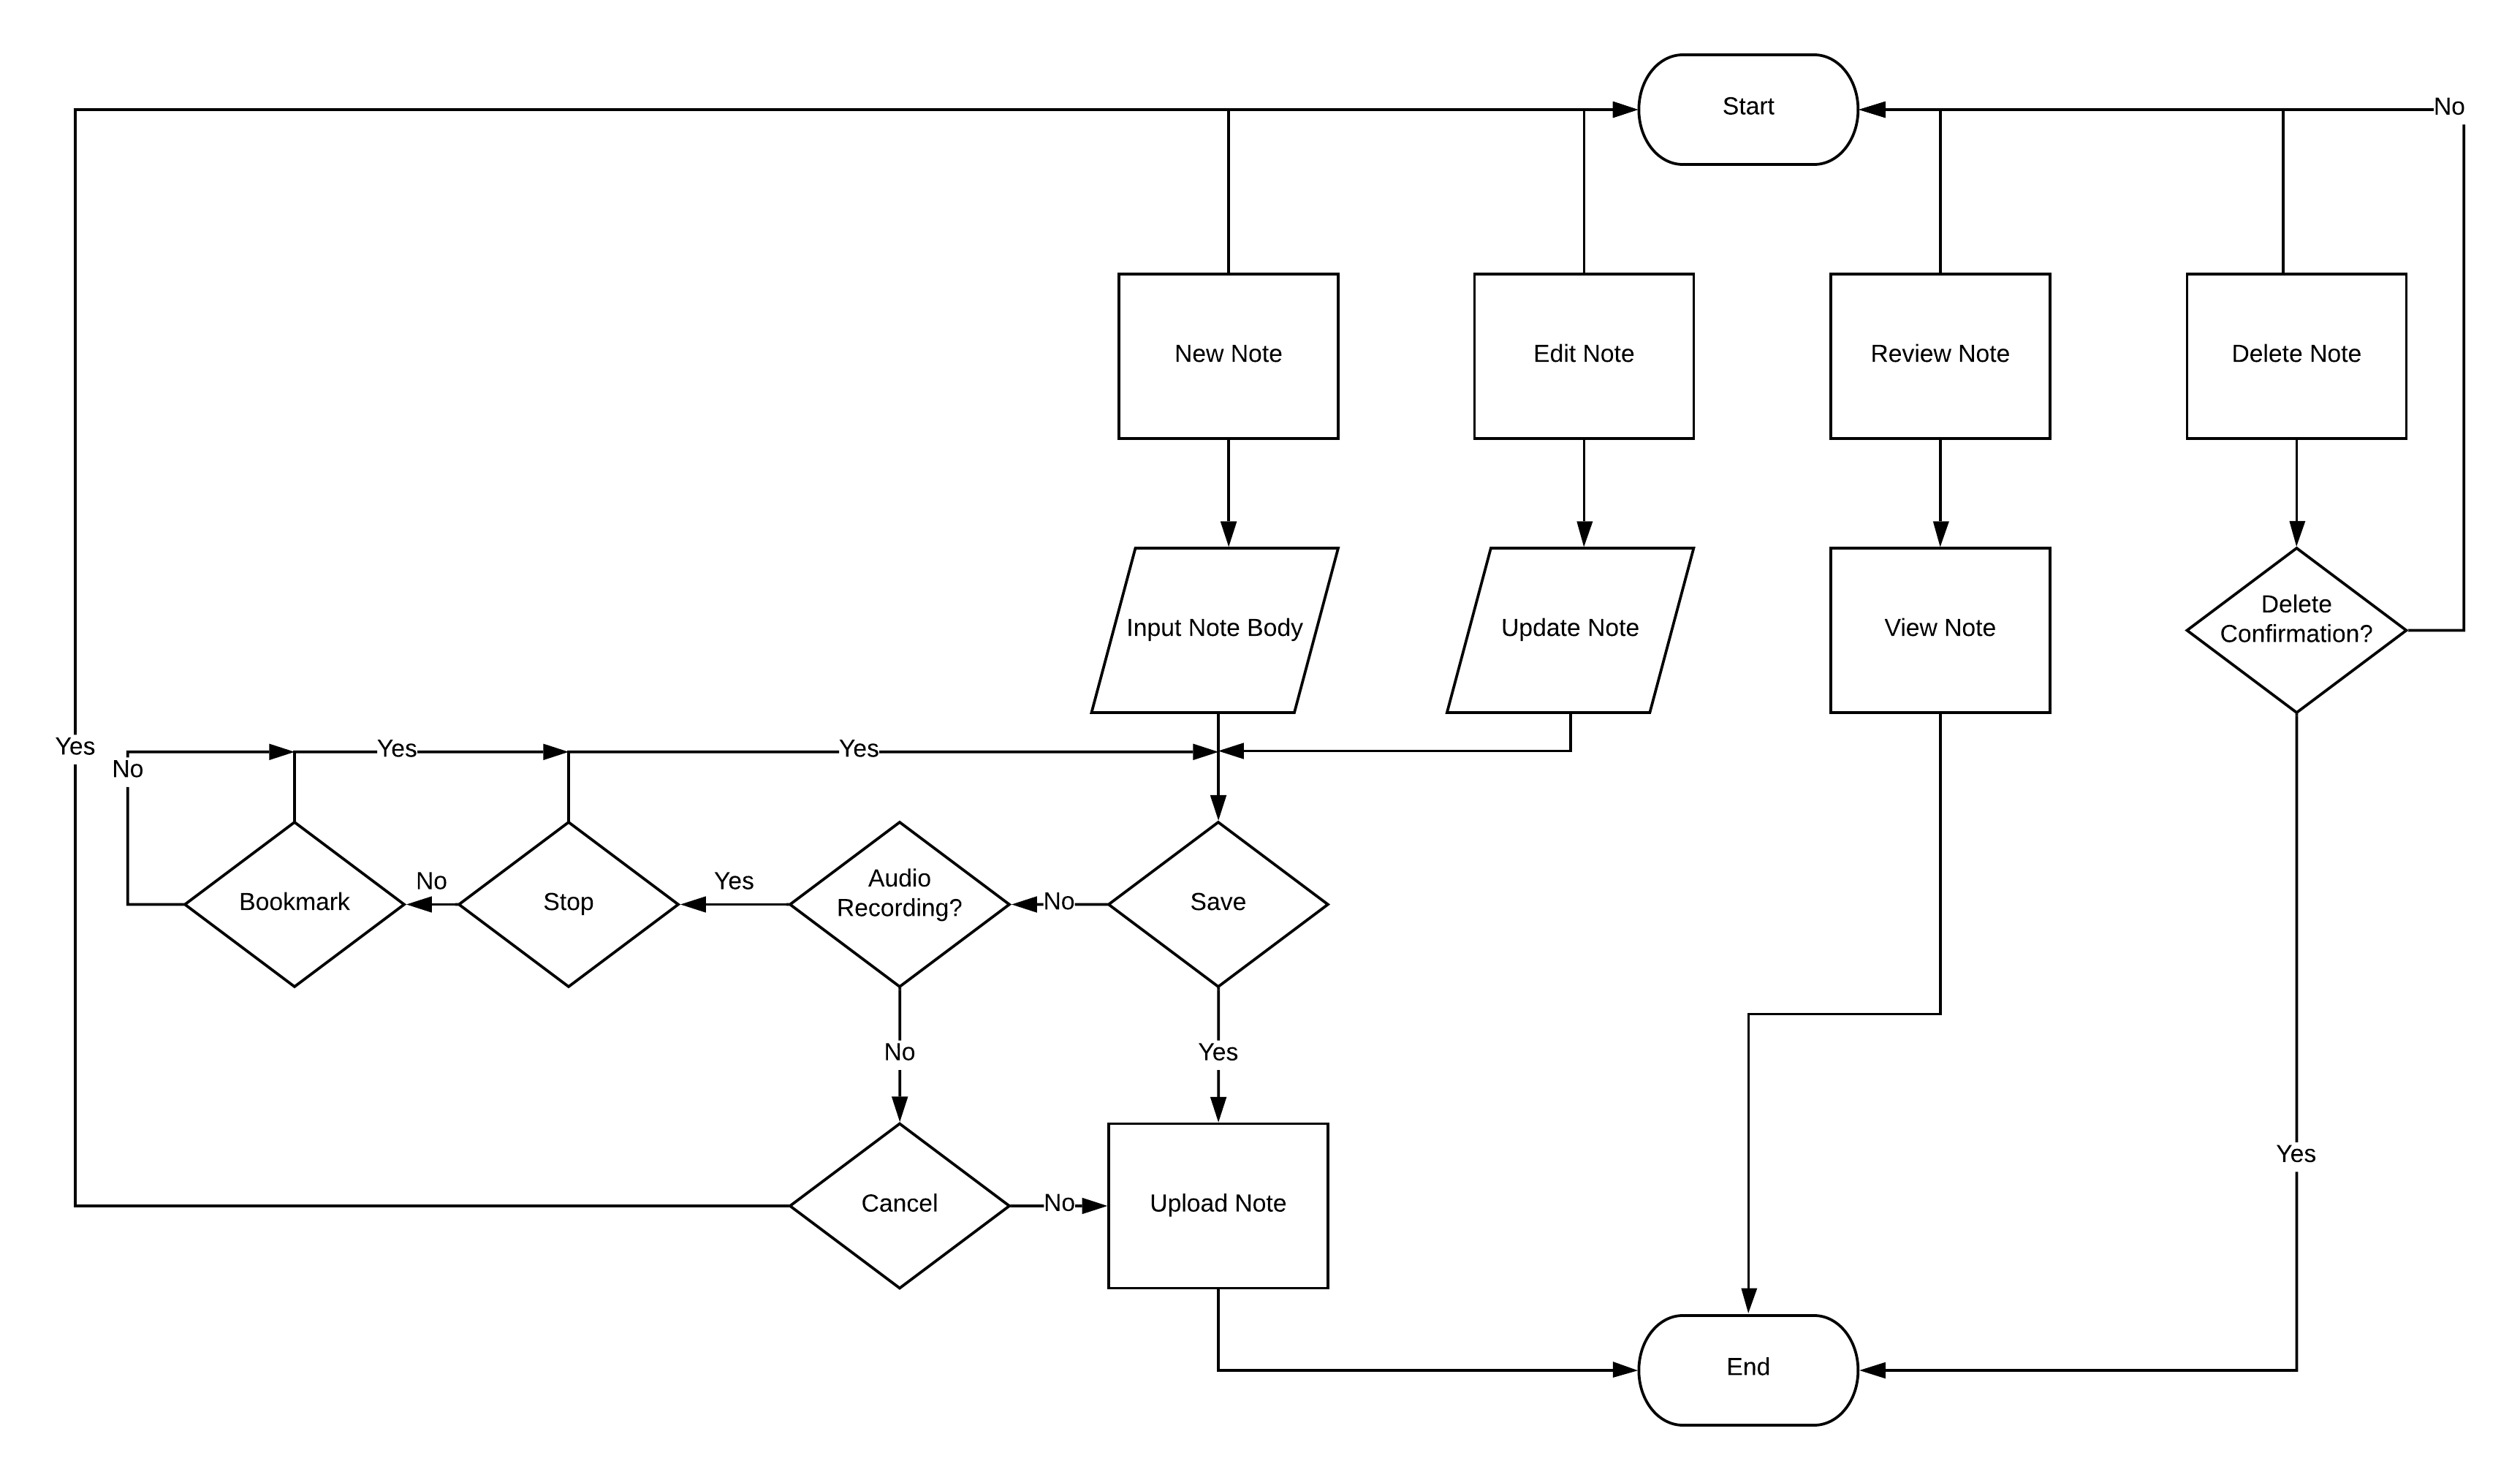
\includegraphics[width=7in]{/ActivityDiagram.png}}
			\end{center}
			\caption[Activity Diagram]{Activity Diagram}
		\end{figure}

		\begin{figure}[H]
			\begin{center}
	 		 	\makebox[\textwidth]{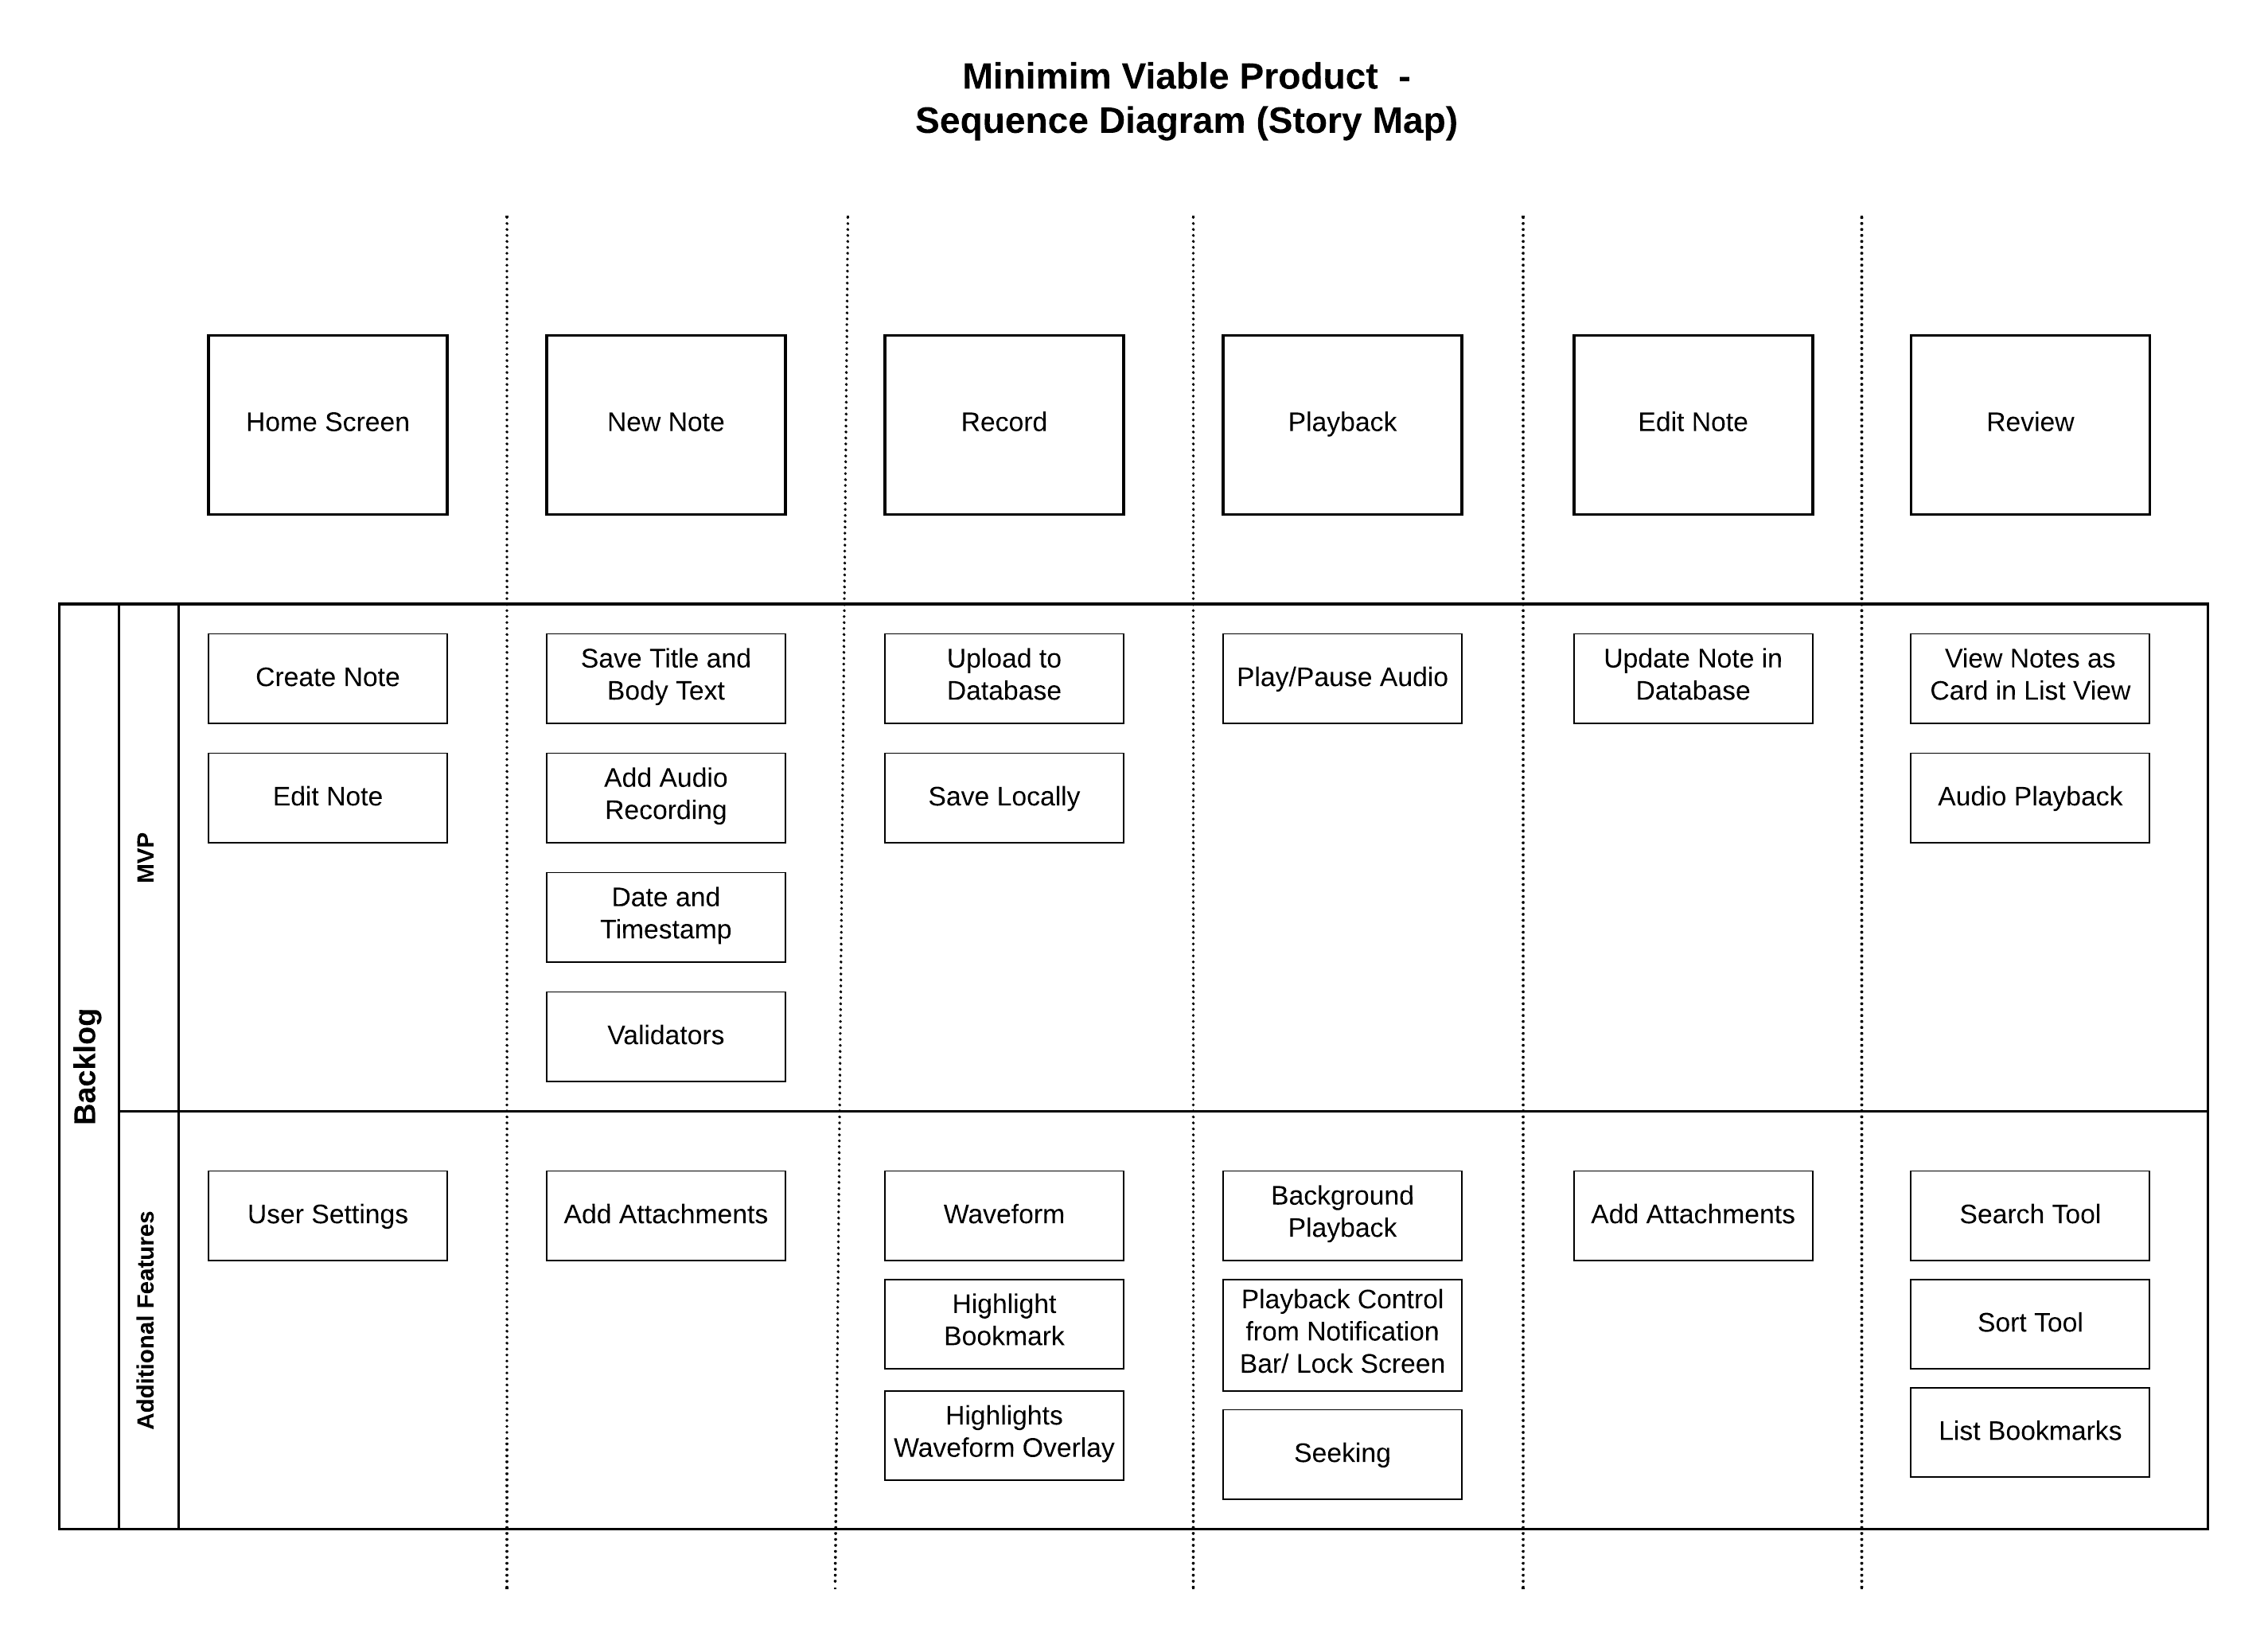
\includegraphics[width=7in]{/SequenceDiagram.png}}
			\end{center}
			\caption[MVP - Sequence Diagram]{MVP - Sequence Diagram}
		\end{figure}

	\chapter{Bugs and Solutions}
		\begin{center}
			\begin{figure}[H]
				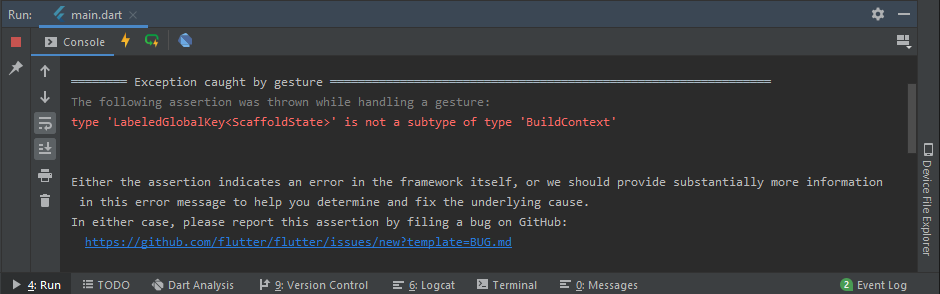
\includegraphics[width=6in]{/bug_1.png}
				\caption[Bug 1: Issue with Scaffold - Displaying the structure of the application]{Bug 1: Issue with Scaffold - Displaying the structure of the application}
			\end{figure}
			\begin{figure}[H]
				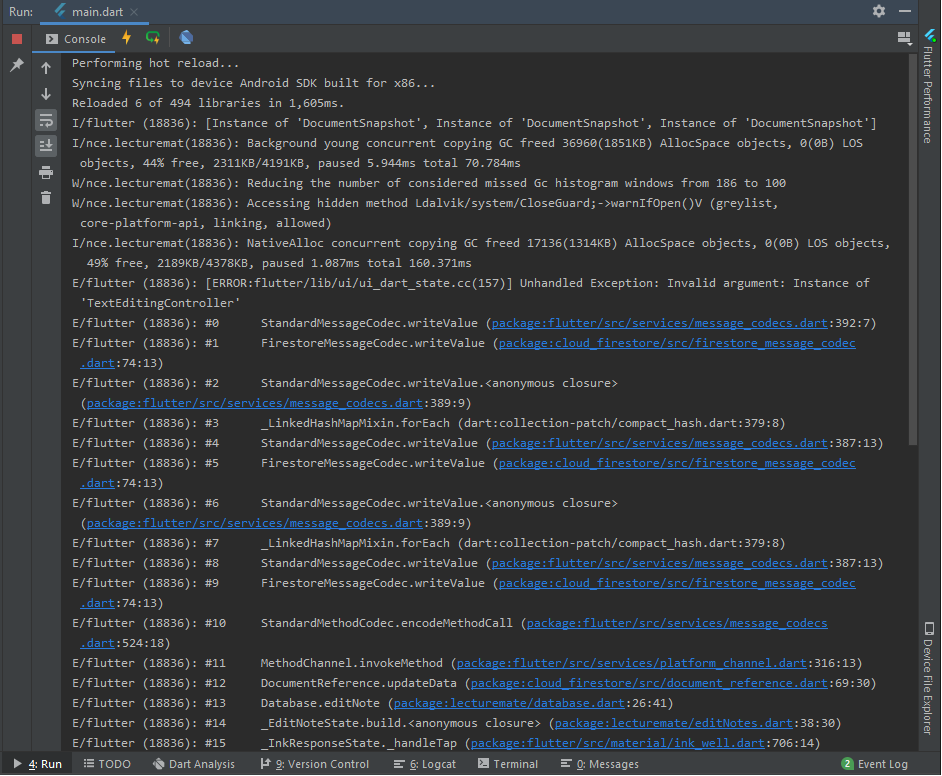
\includegraphics[width=6in]{/bug_2.png}
				\caption[Bug 2: Issue with retrieving data from Firebase]{Bug 2: Issue with retrieving data from Firebase}
			\end{figure}
		\end{center}
	\chapter{Surveys and Results}

		\begin{figure}[H]%
			\centering
			\subfloat[Survey Page 1]{{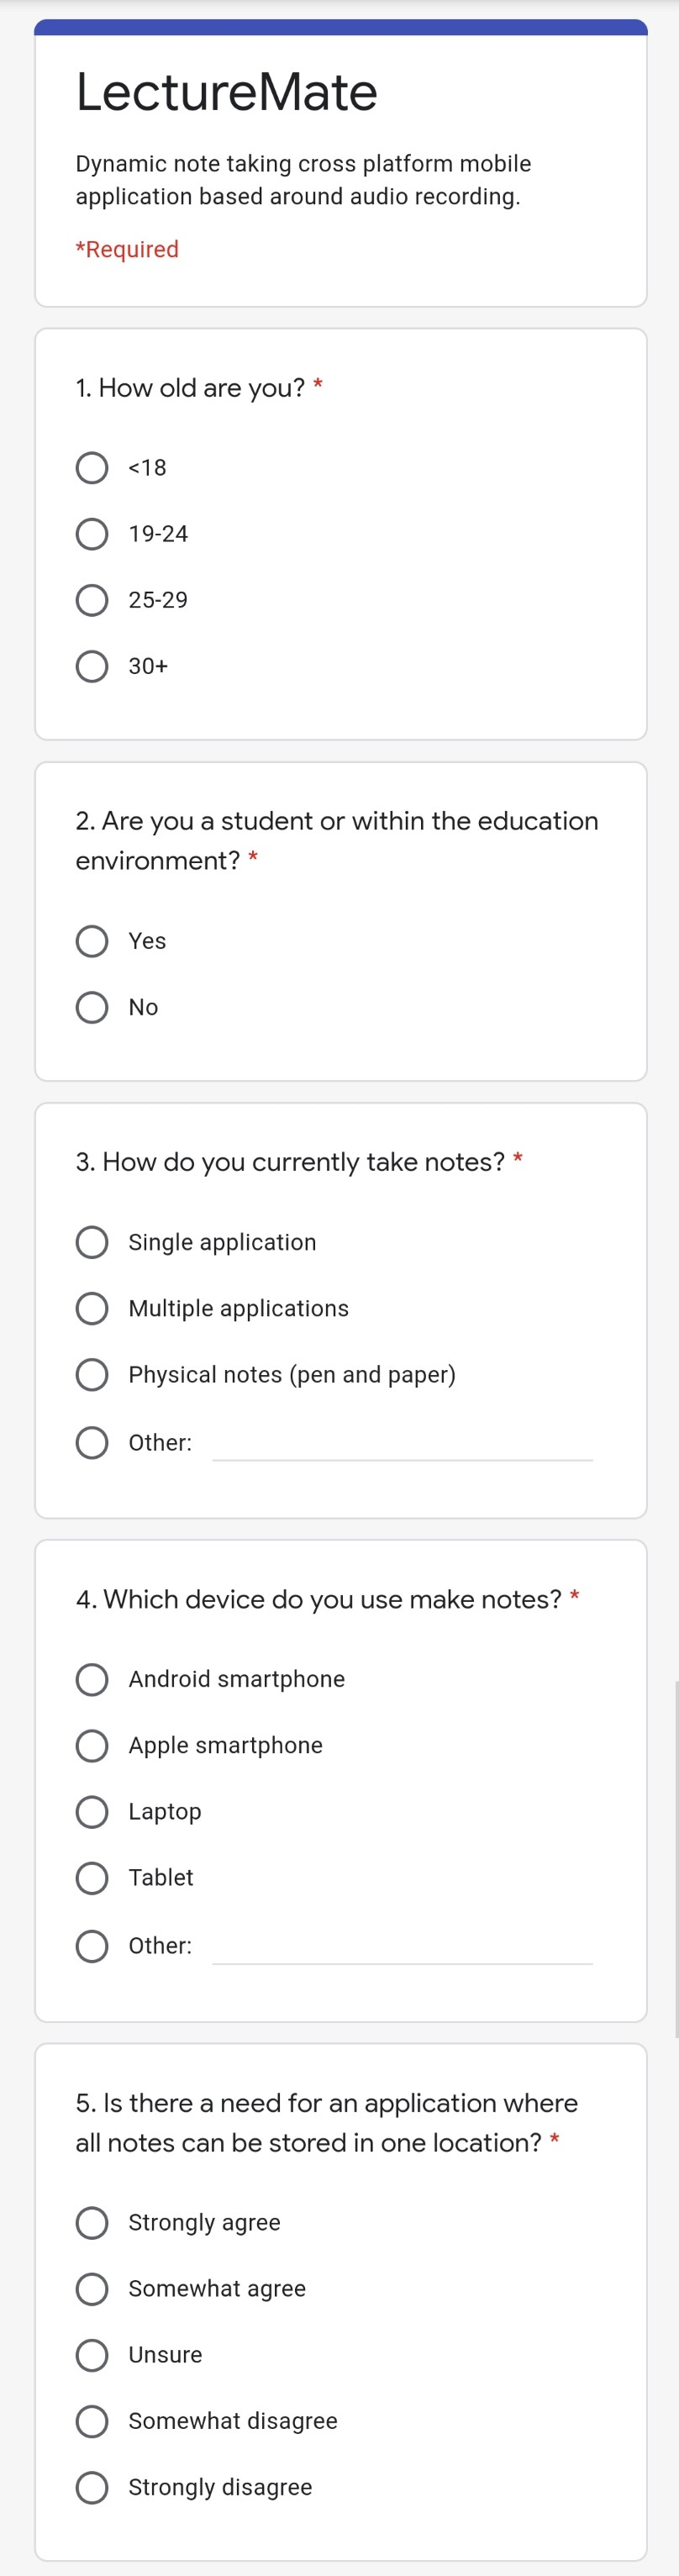
\includegraphics[width=1.75in]{Survey1.jpg} }}%
			\qquad
			\subfloat[Survey Page 2]{{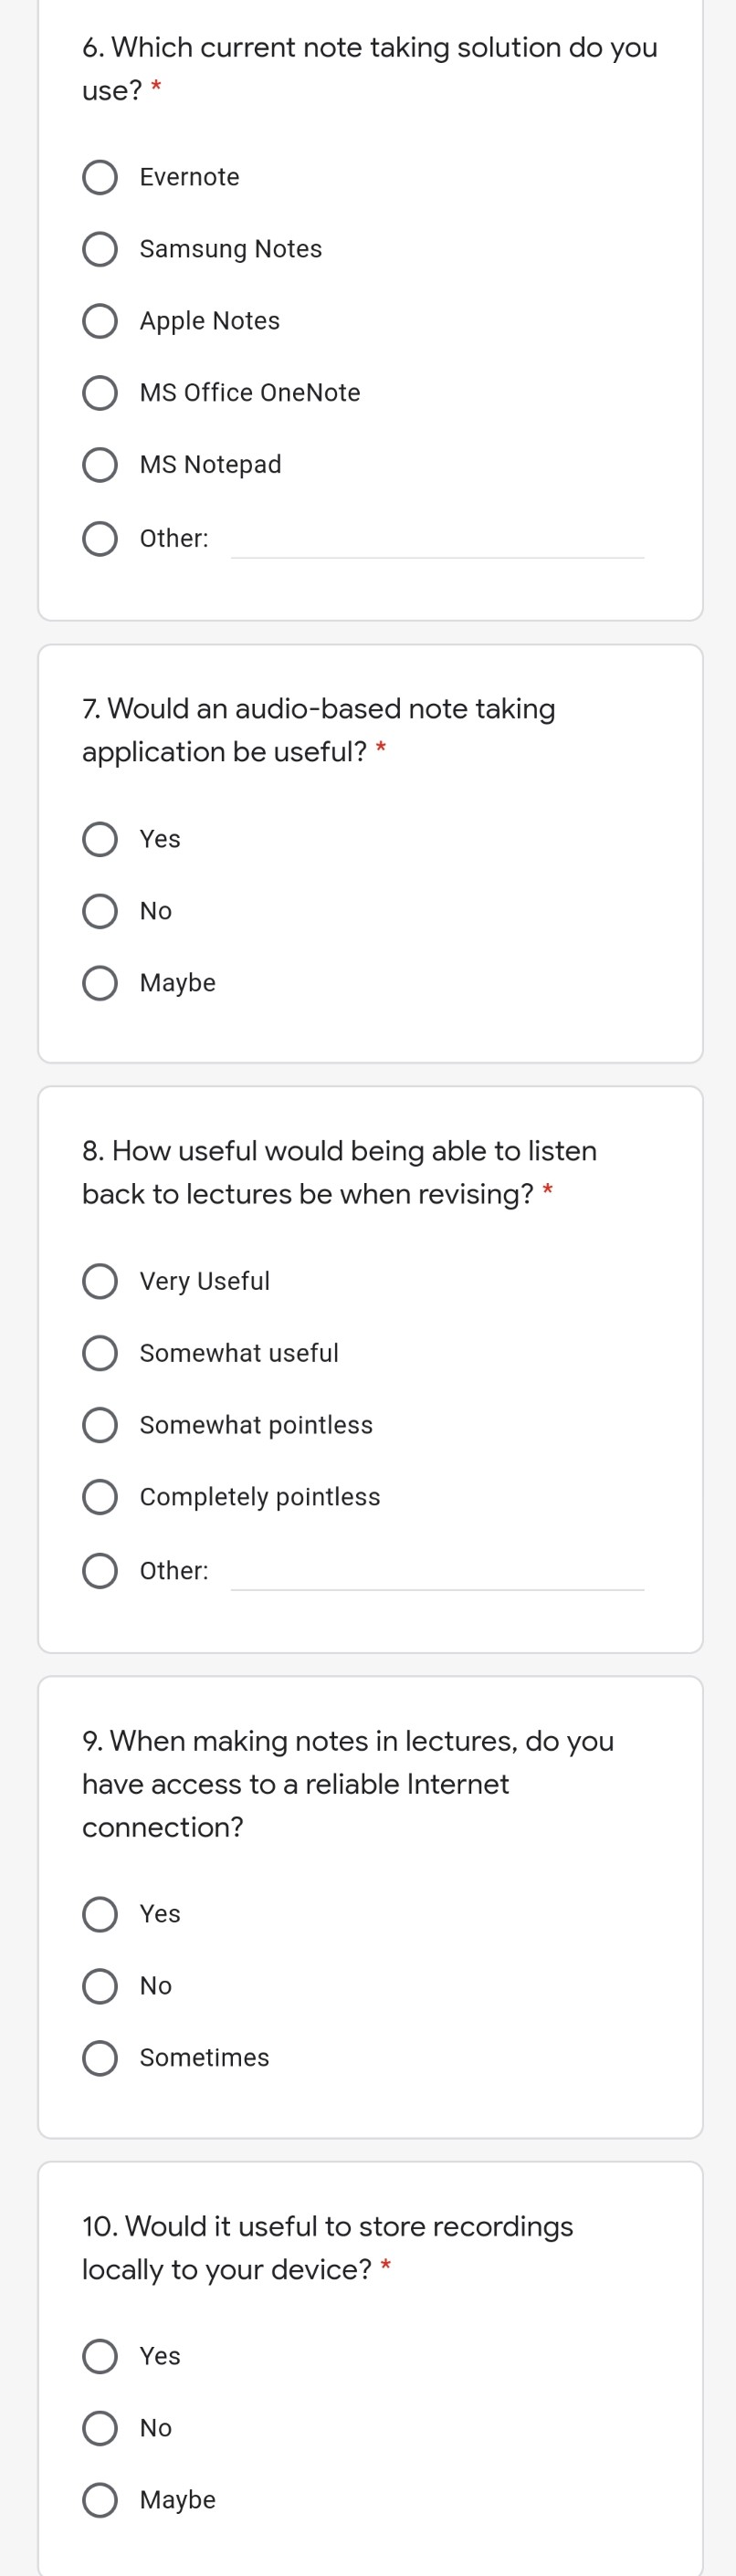
\includegraphics[width=1.75in]{Survey2.jpg} }}%
			\caption{Survey}%
			\label{Survey}%
			The survey can be found at: \url{https://forms.gle/1DZCzhv5XxWYGPT8A}
		\end{figure}

		\begin{figure}[H]%
			\centering
			\subfloat[Survey Results 1]{{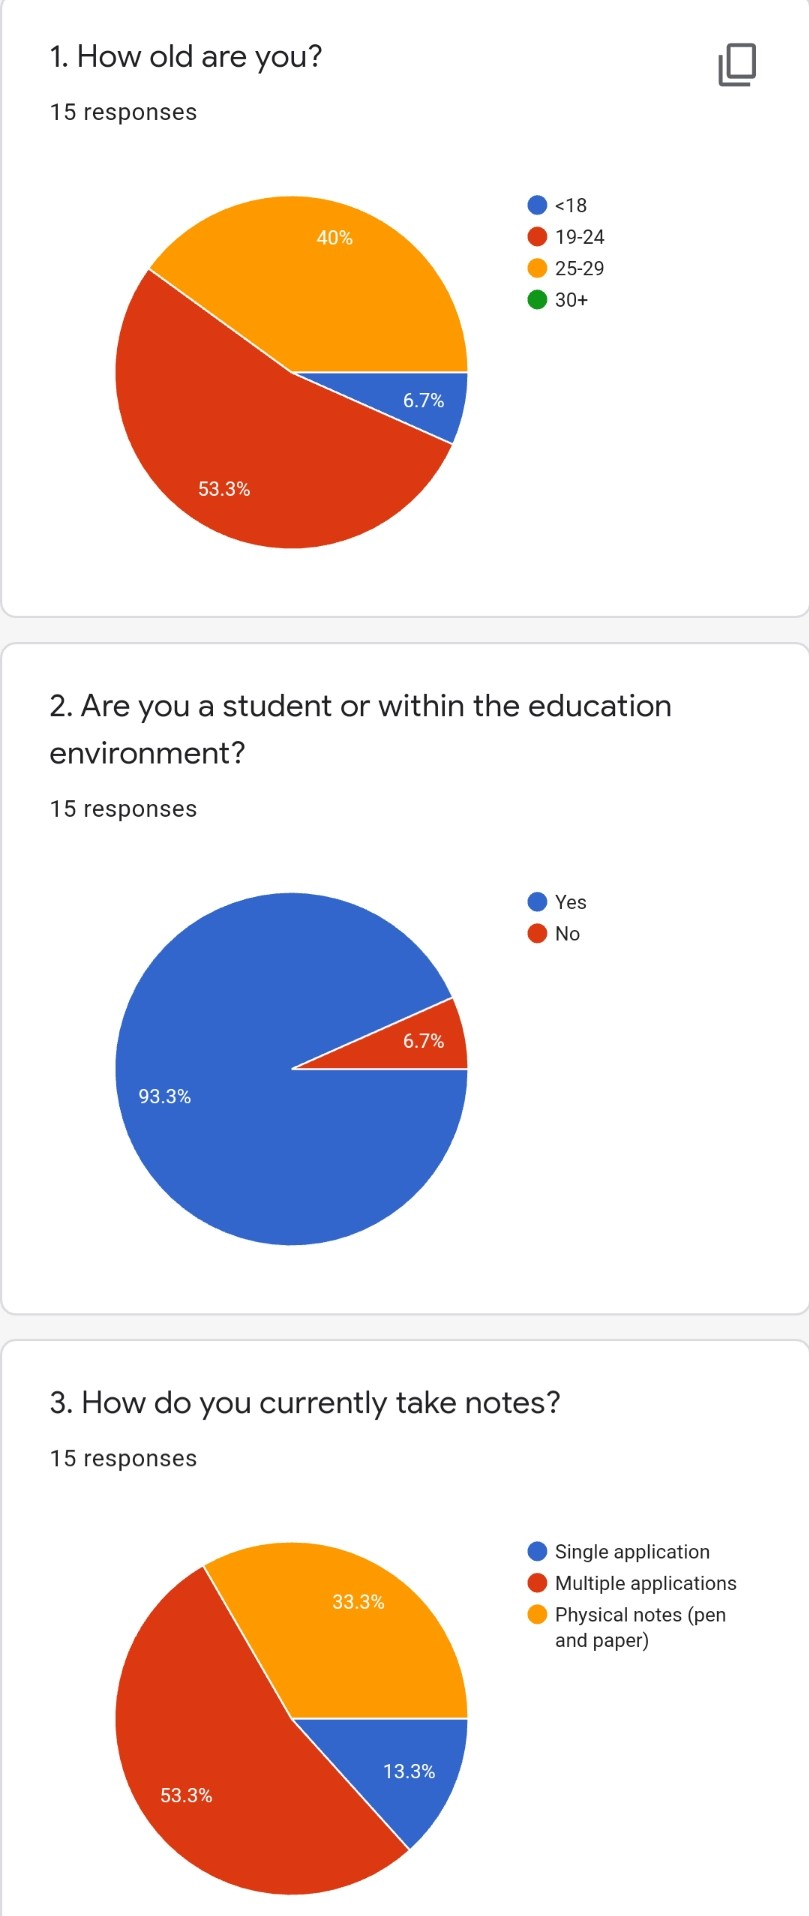
\includegraphics[width=1.75in]{Results.jpg} }}%
			\qquad
			\subfloat[Survey Results 2]{{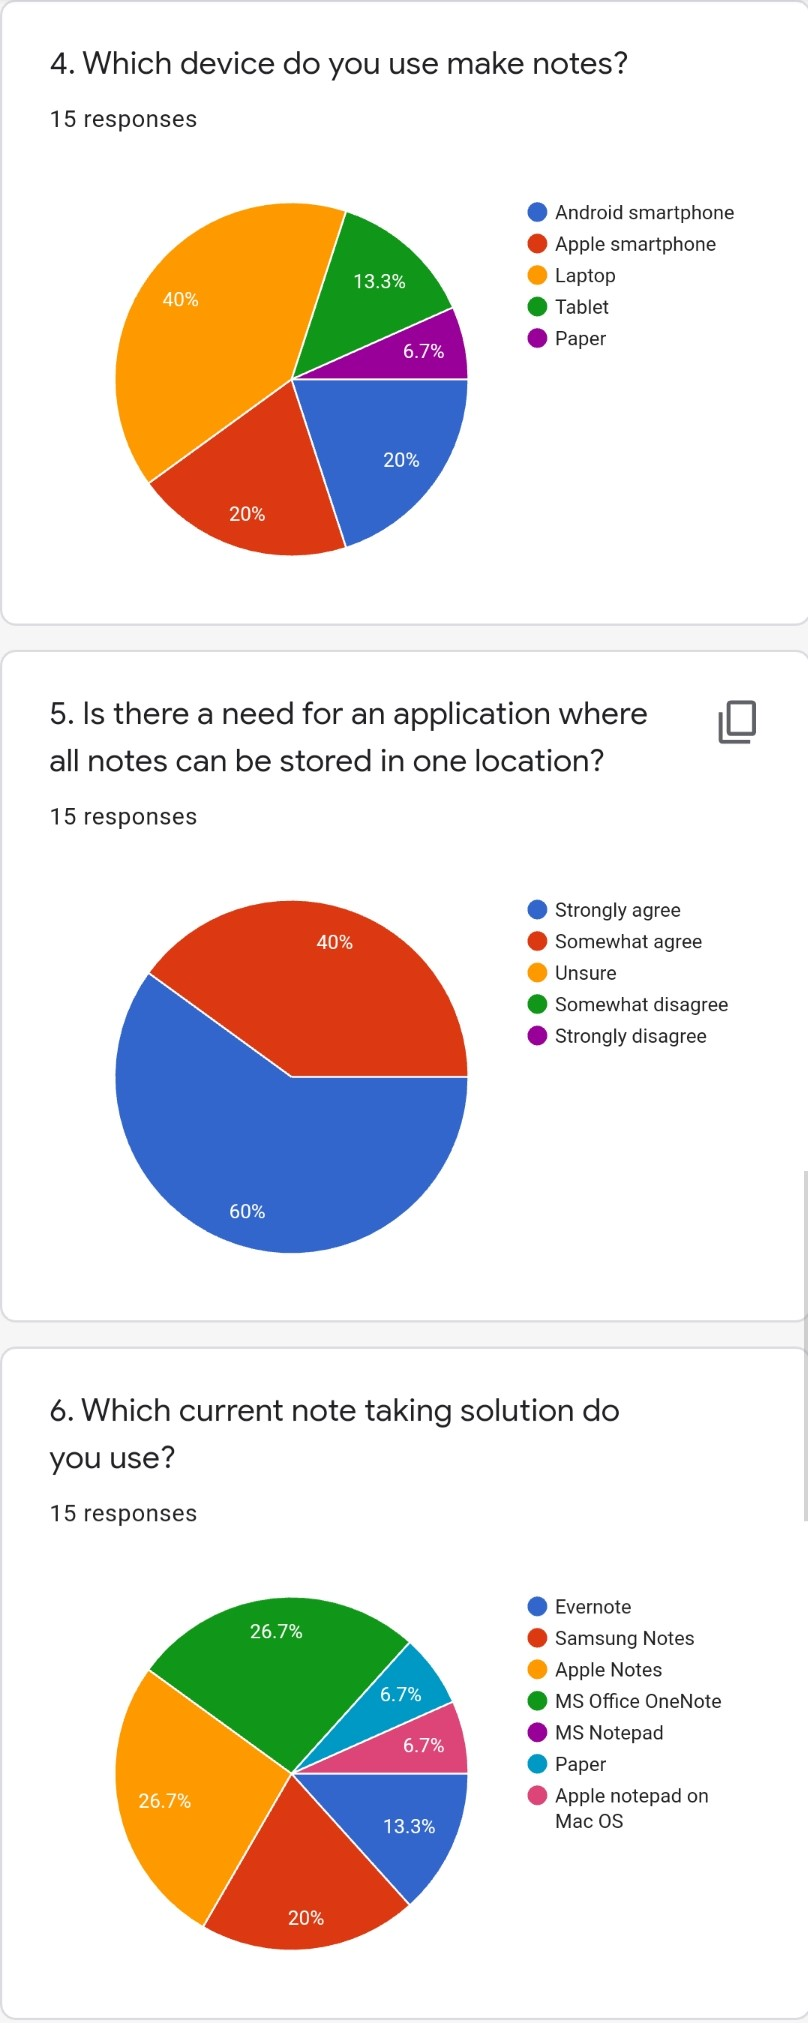
\includegraphics[width=1.75in]{Results2.jpg} }}%
			\qquad
			\subfloat[Survey Results 3]{{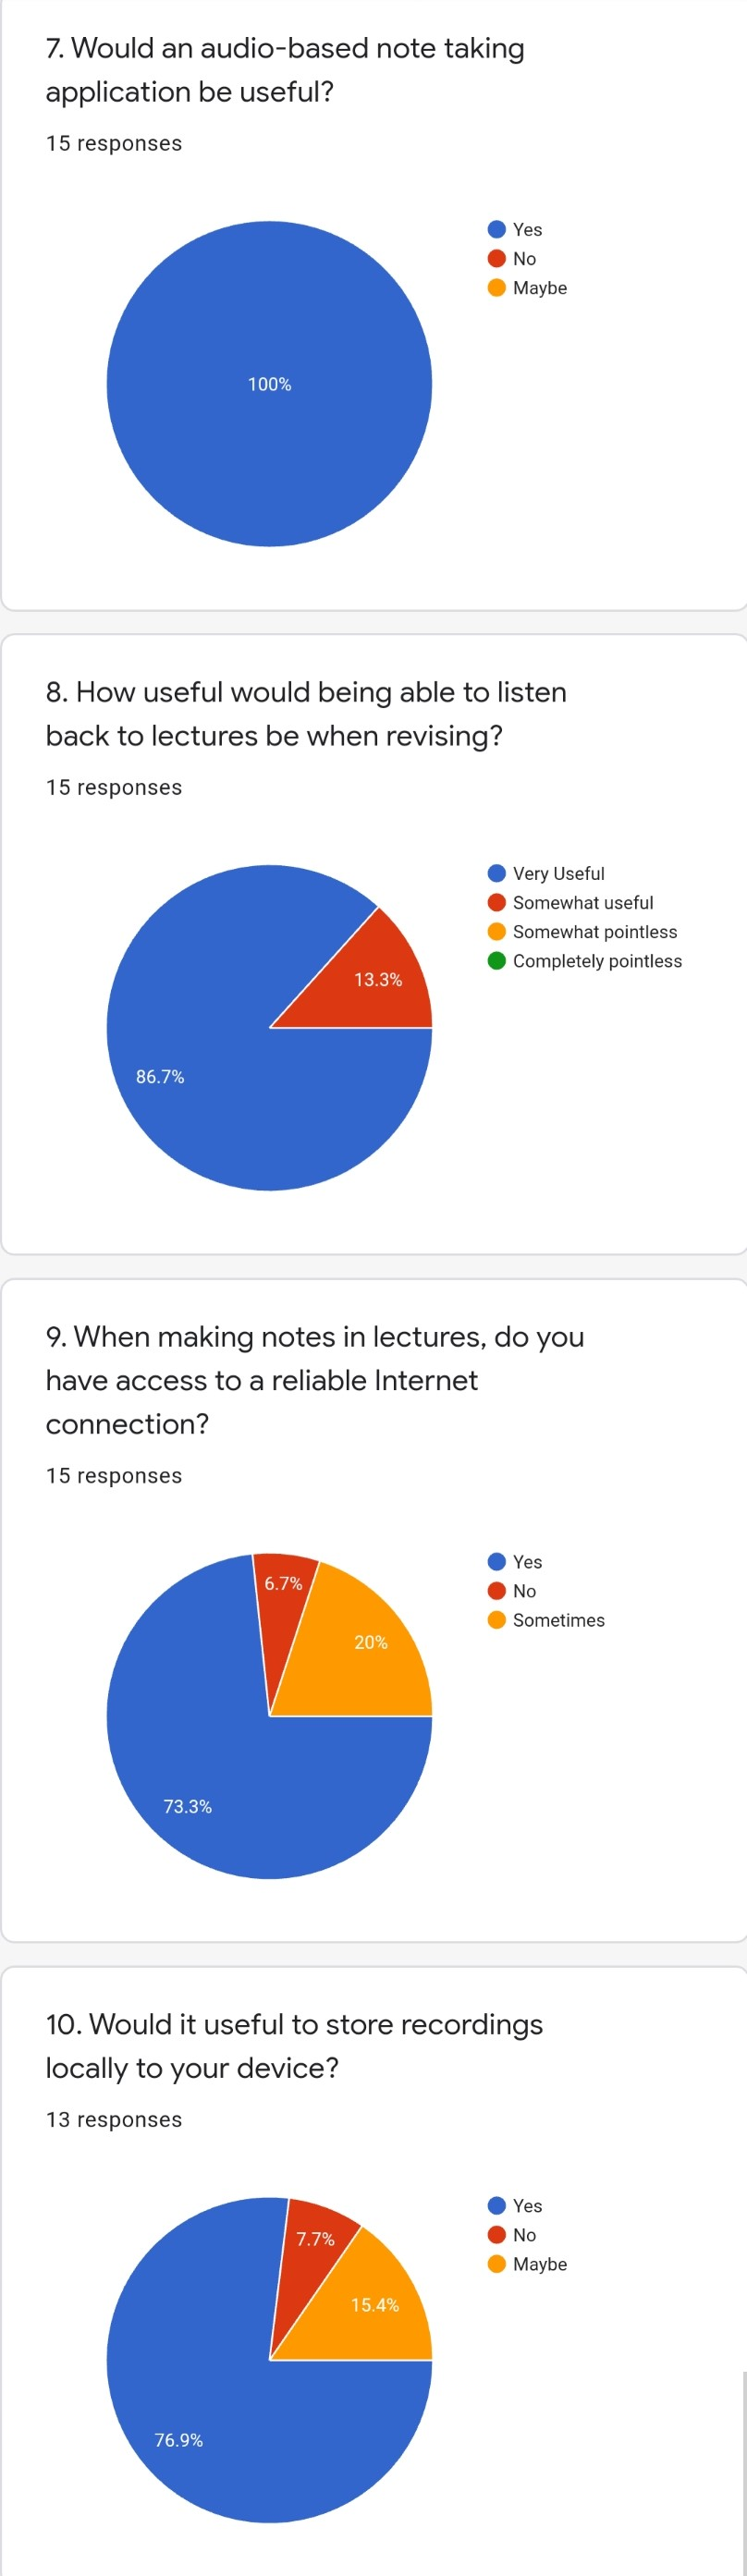
\includegraphics[width=1.75in]{Results3.jpg} }}%
			\caption{Survey Results}%
			\label{Survey Results}%
		\end{figure}

	\chapter{Prototypes}

%--------------------------Paper Prototypes--------------------------------

		\begin{figure}[H]%
		    \centering
		    \subfloat[Splash Page]{{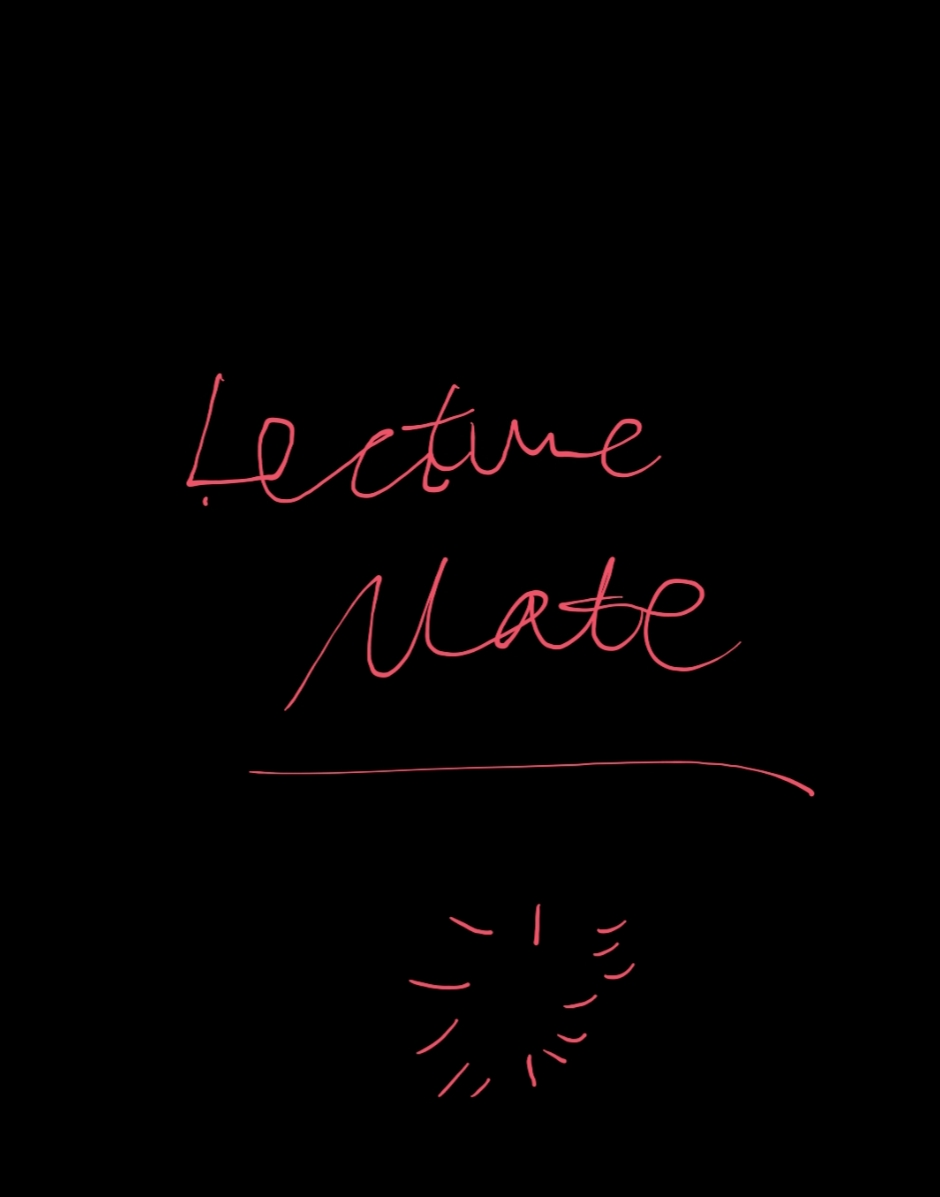
\includegraphics[width=2in]{0.jpeg} }}%
		    \qquad
		    \subfloat[Home Page]{{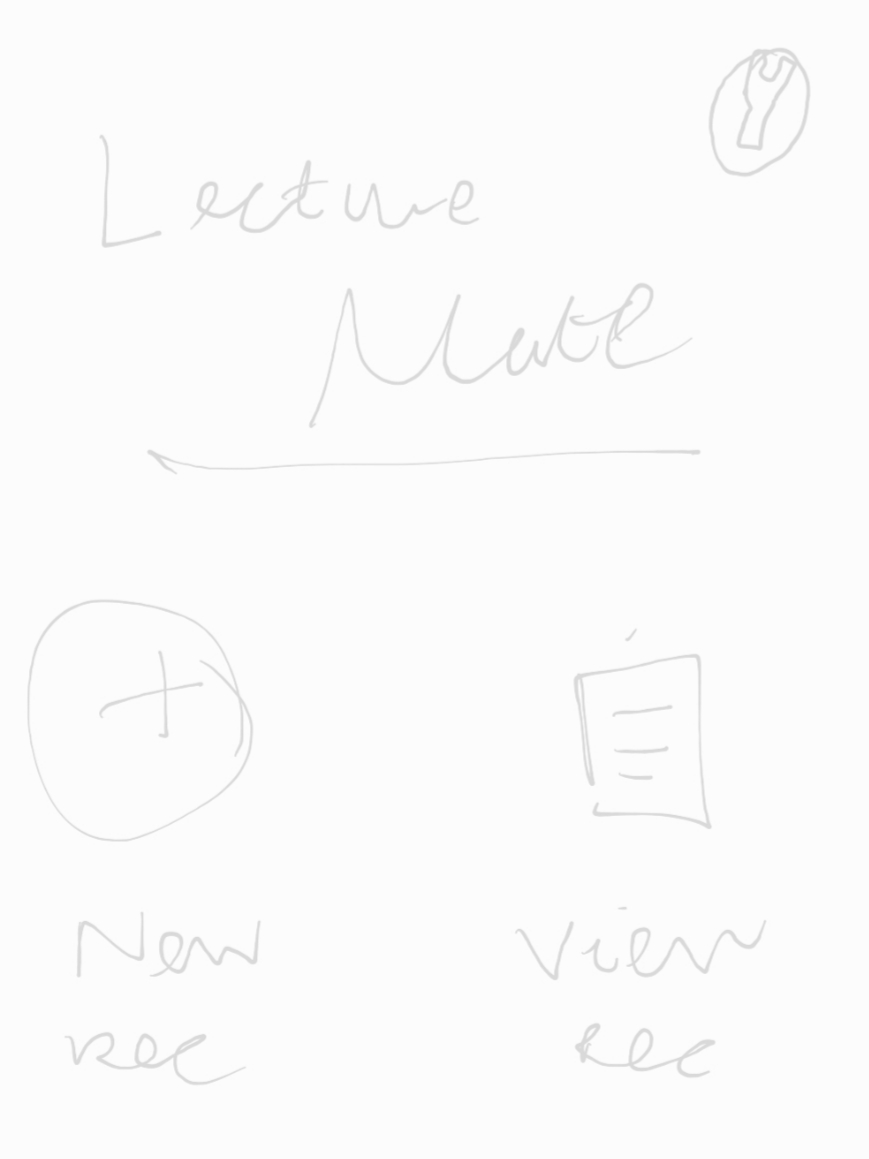
\includegraphics[width=2in]{1.jpeg} }}%
		    \qquad
		    \subfloat[New Recording]{{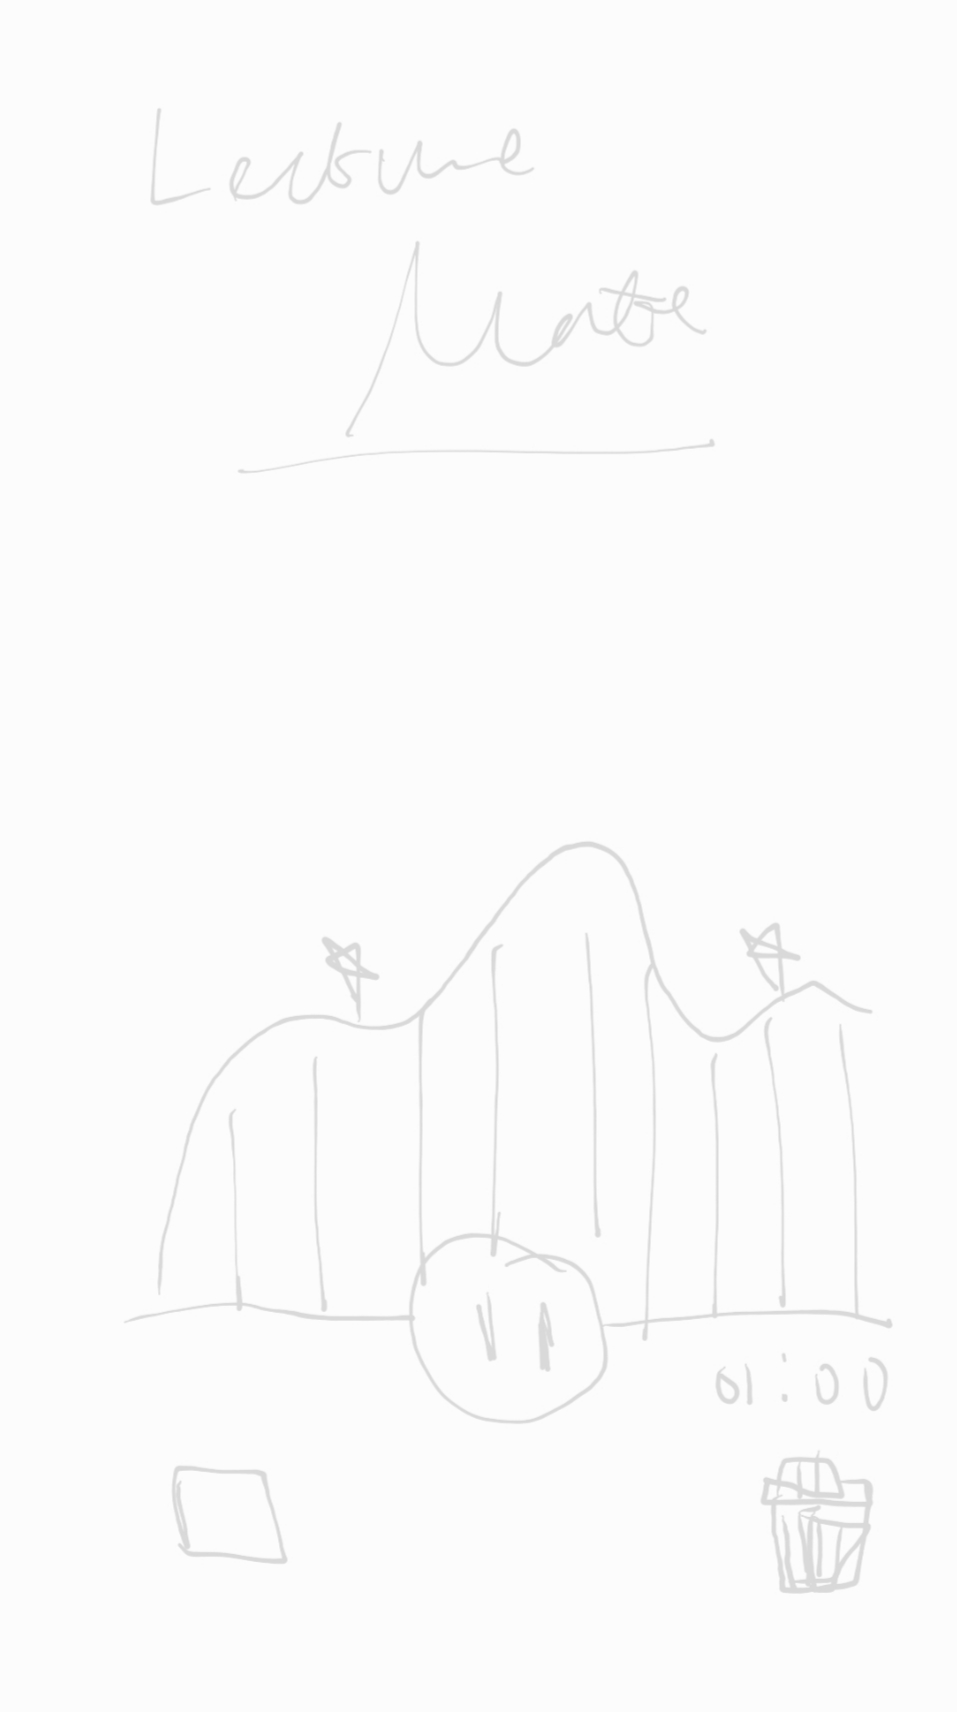
\includegraphics[width=2in]{2.jpeg} }}%
		    \qqua
		    \subfloat[List Notes]{{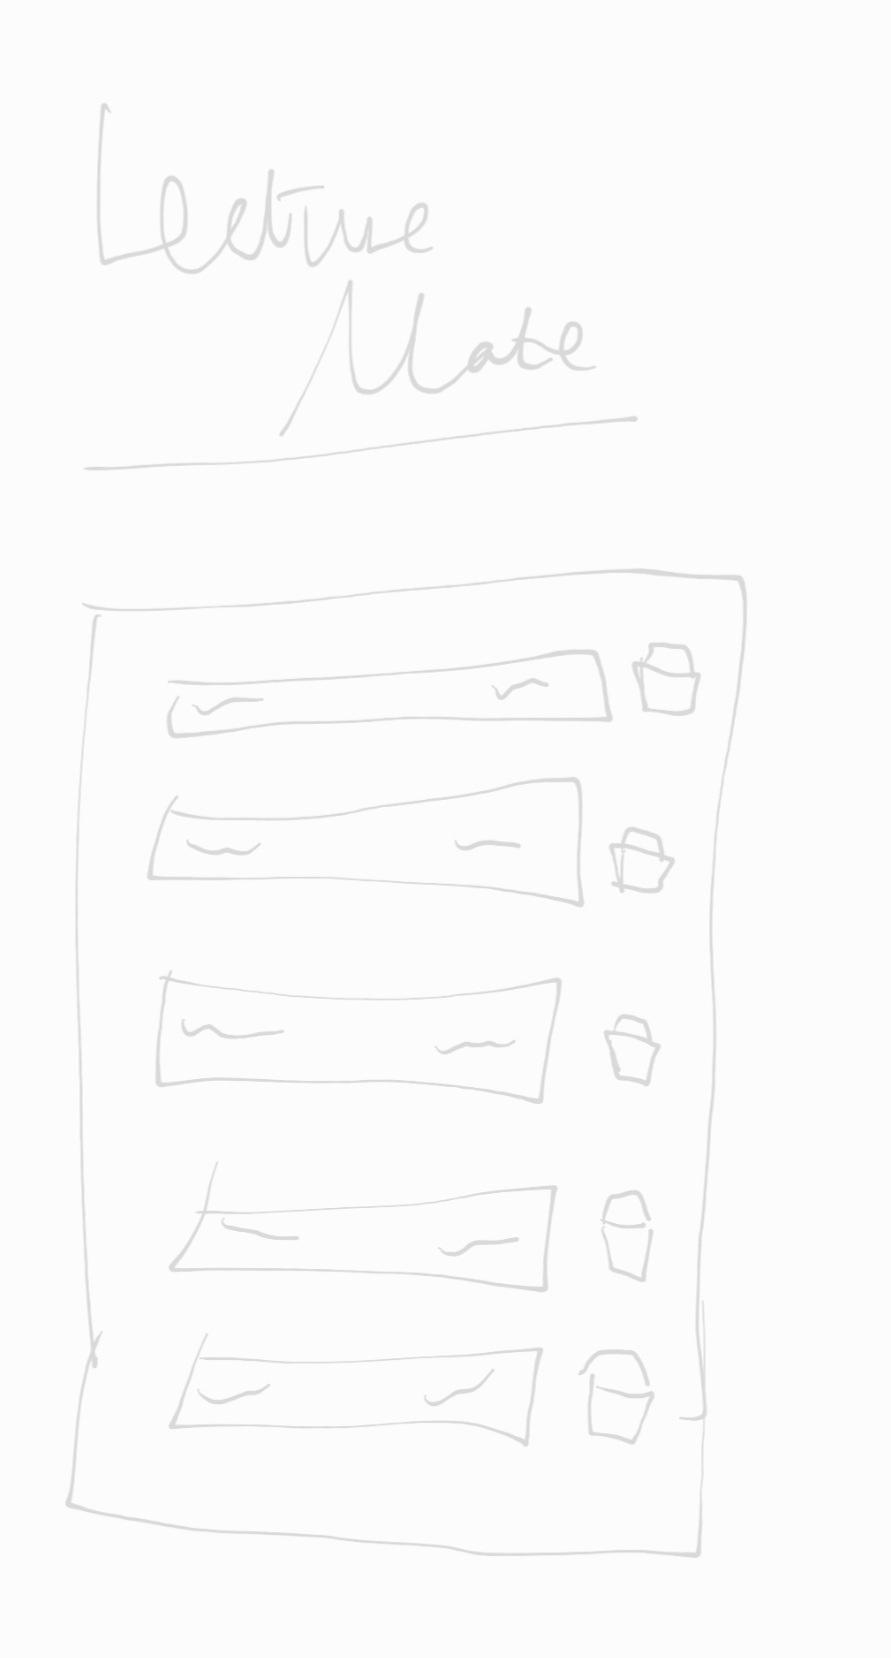
\includegraphics[width=2in]{3.jpeg} }}%
		    \caption{Paper Prototypes}%
		    \label{Paper Prototypes}%
		\end{figure}

		\begin{figure}[H]%
		    \centering
		    \subfloat[Delete Note Dialog]{{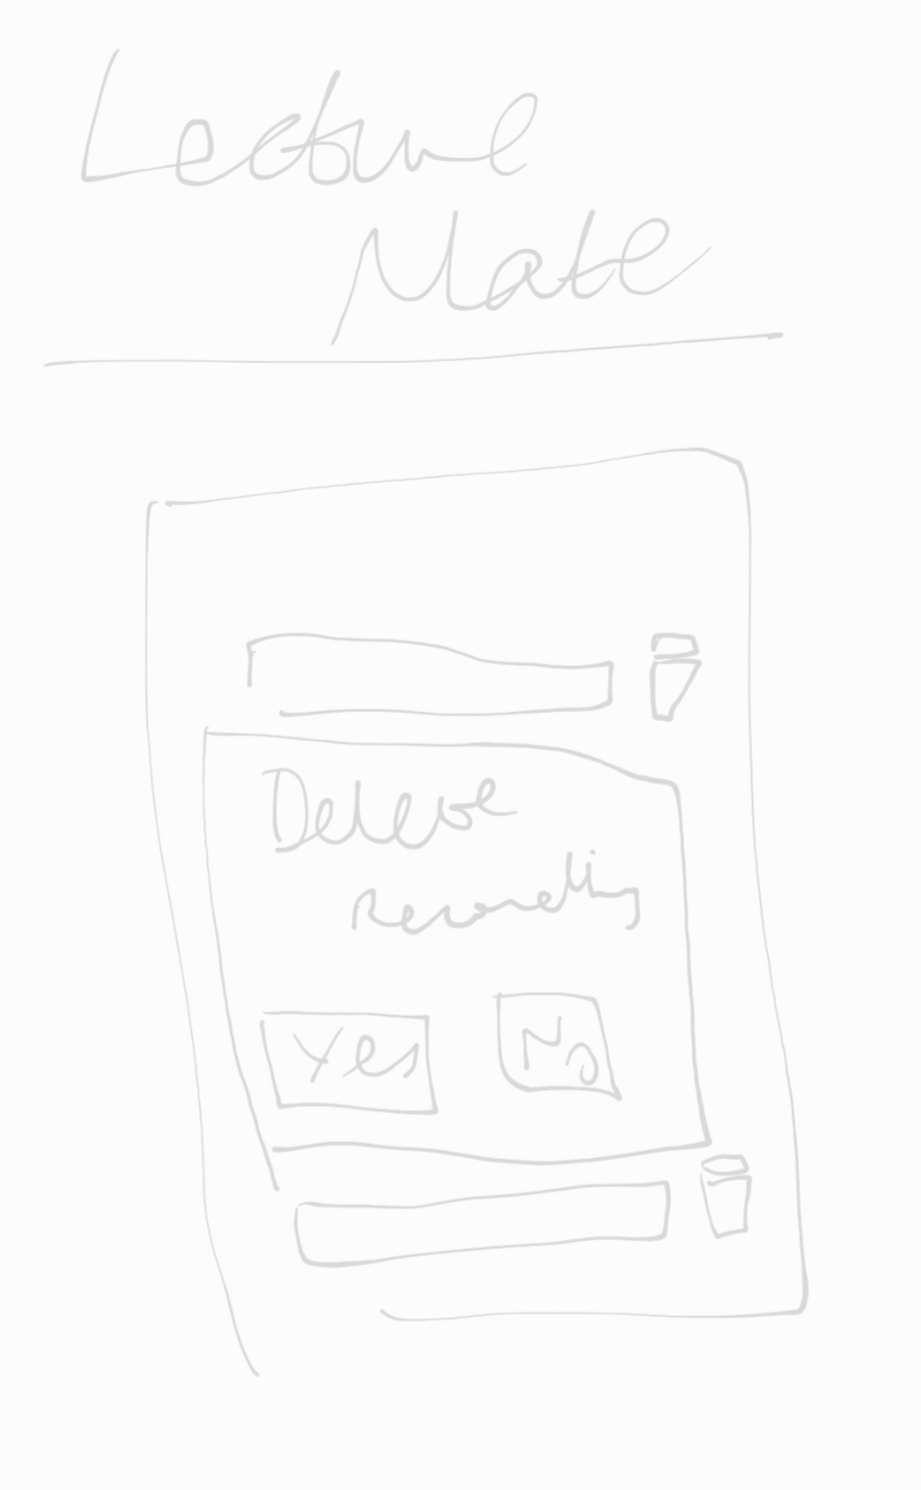
\includegraphics[width=2in]{4.jpeg} }}%
		    \qquad
		    \subfloat[View Note]{{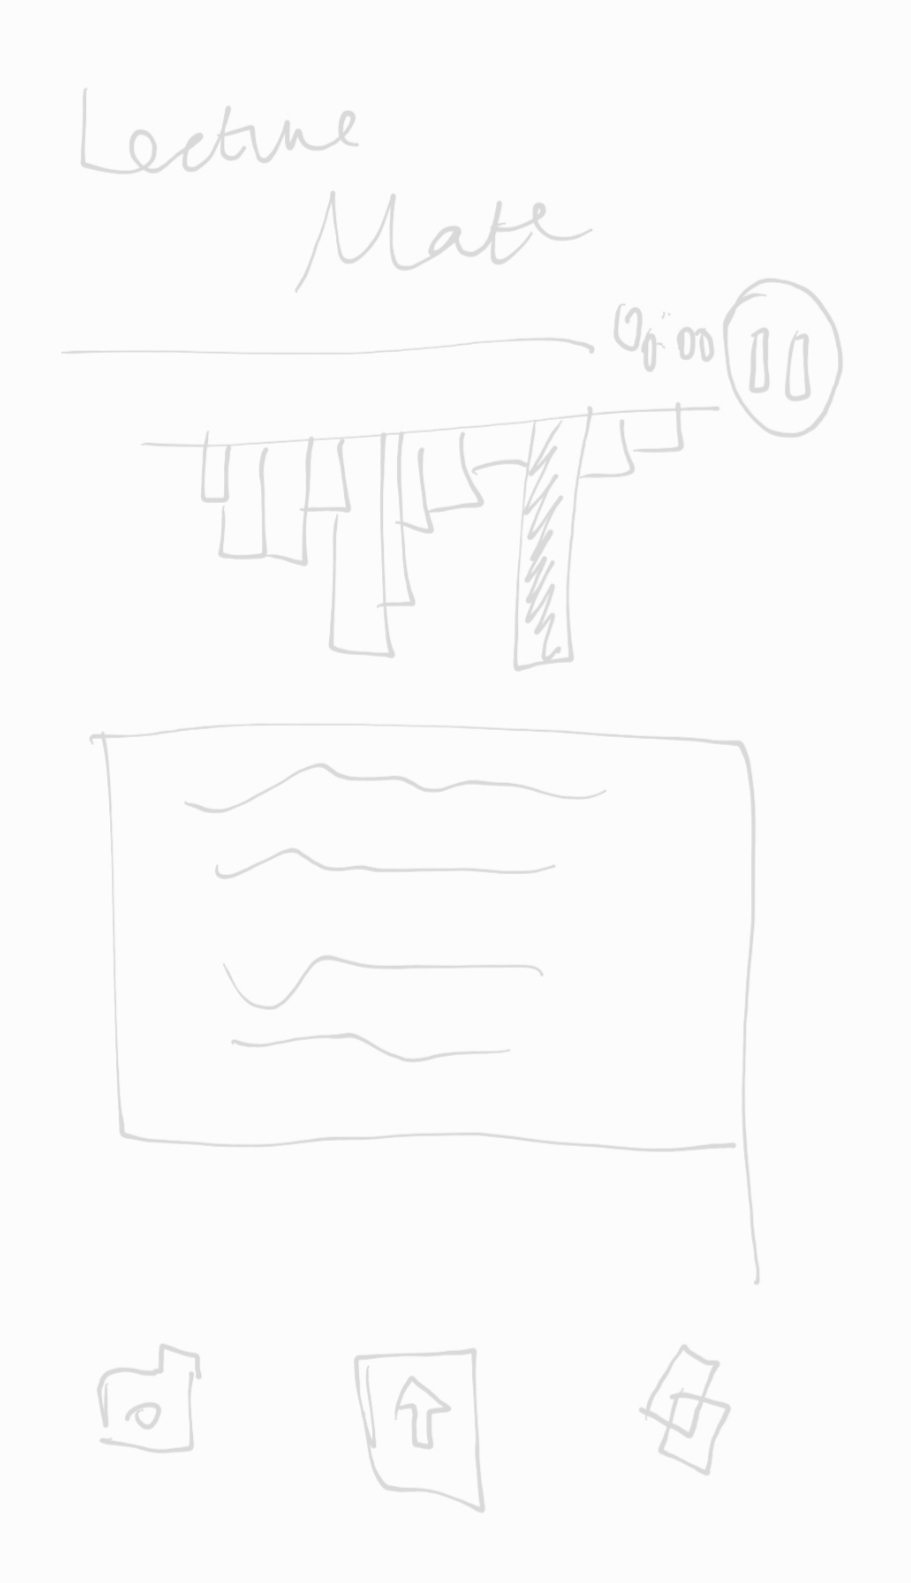
\includegraphics[width=2in]{5.jpeg} }}%
		    \caption{Paper Prototypes (Continued)}%
		    \label{Paper Prototypes (Continued)}%
		\end{figure}

%--------------------------High Fidelity Prototypes----------------------------

		\begin{figure}[H]%
		    \centering
		    \subfloat[Splash Page]{{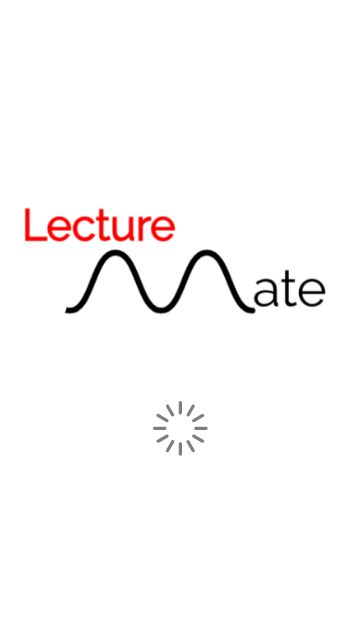
\includegraphics[width=2in]{LectureMate_Splash.png} }}%
		    \qquad
		    \subfloat[Home Page]{{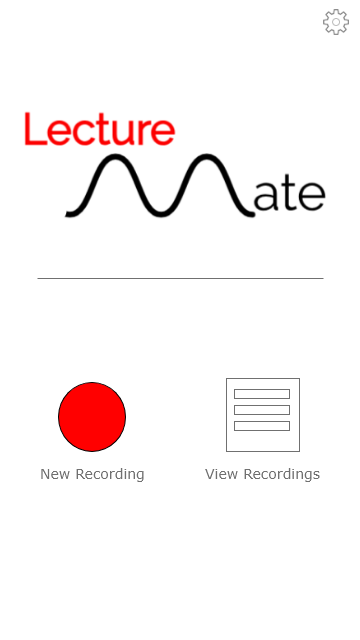
\includegraphics[width=2in]{LectureMate_Home.png} }}%
		    \qquad
		    \subfloat[New Recording]{{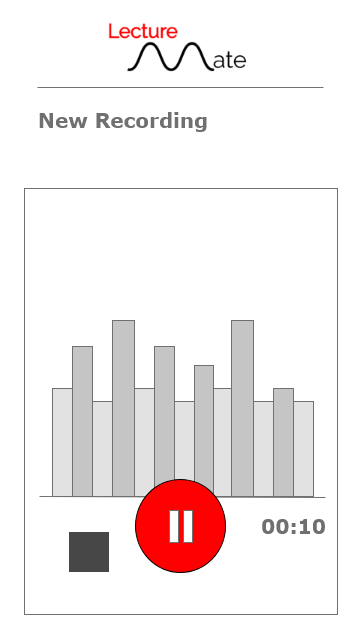
\includegraphics[width=2in]{LectureMate_New.png} }}%
		    \qquad
		    \subfloat[List Notes]{{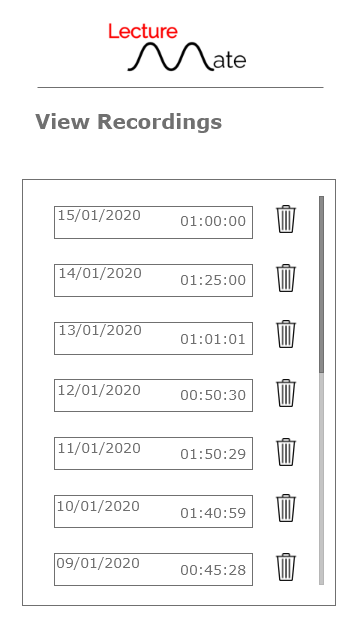
\includegraphics[width=2in]{LectureMate_View.png} }}%
		    \caption{High Fidelity Prototypes}%
		    \label{High Fidelity Prototypes}%
		\end{figure}

		\begin{figure}[H]%
		    \centering
		    \subfloat[Delete Note Dialog]{{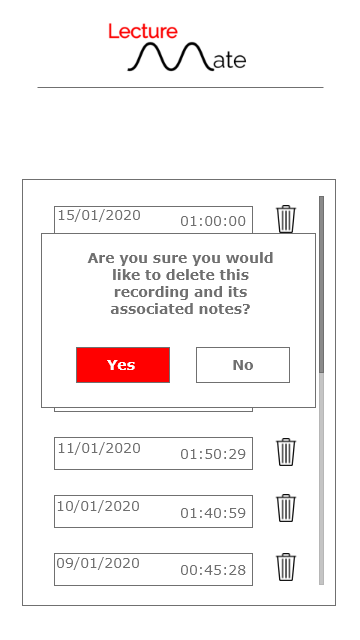
\includegraphics[width=2in]{LectureMate_Delete.png} }}%
		    \qquad
		    \subfloat[View Note]{{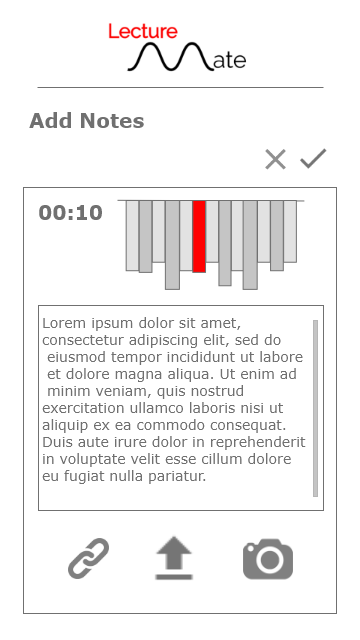
\includegraphics[width=2in]{LectureMate_AddNotes.png} }}%
		    \caption{High Fidelity Prototypes (Continued)}%
		    \label{High Fidelity Prototypes (Continued)}%
		\end{figure}
		
	\chapter{Google Firebase Database}
			\begin{figure}[H]
				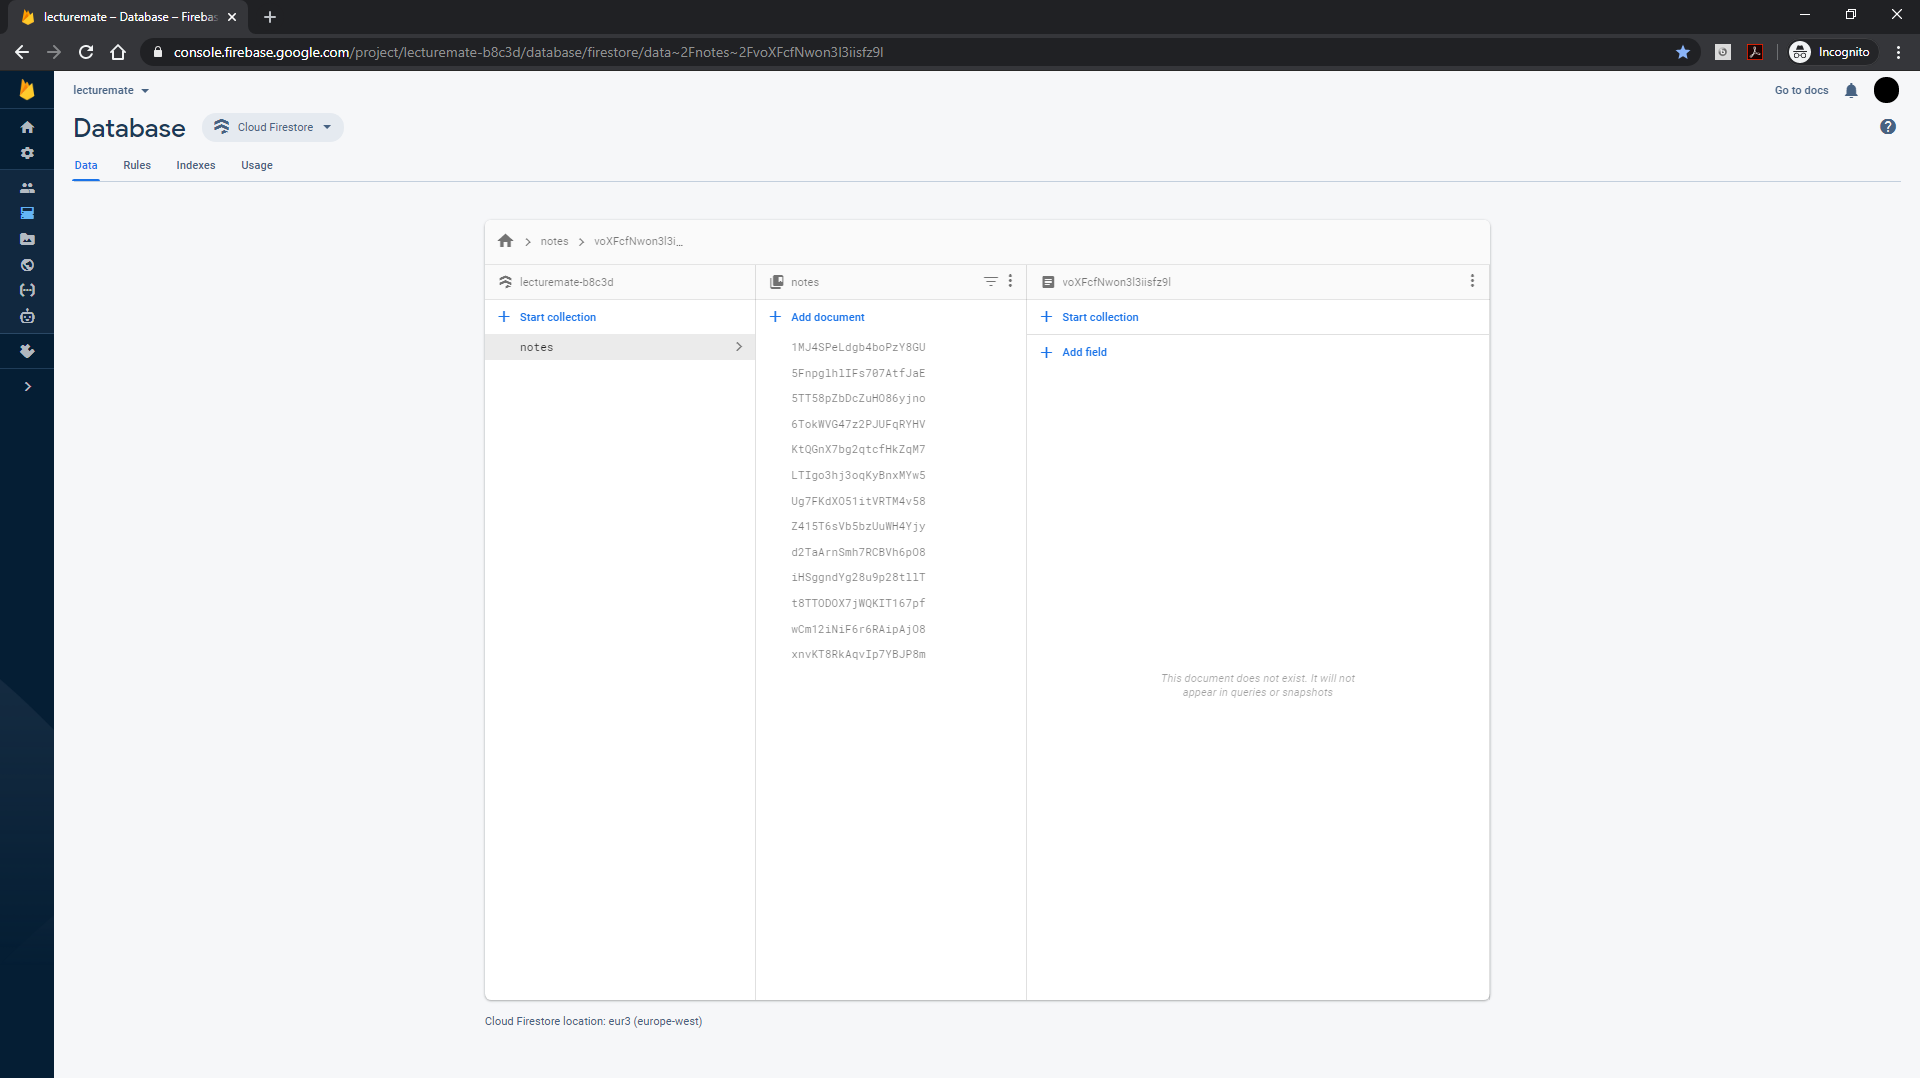
\includegraphics[width=6in]{/Firebase.png}
				\caption[Google Firebase]{Google Firebase}
			\end{figure}
			
	\chapter{Project Management}
		\section{Gantt Chart}
			\begin{figure}[H]
				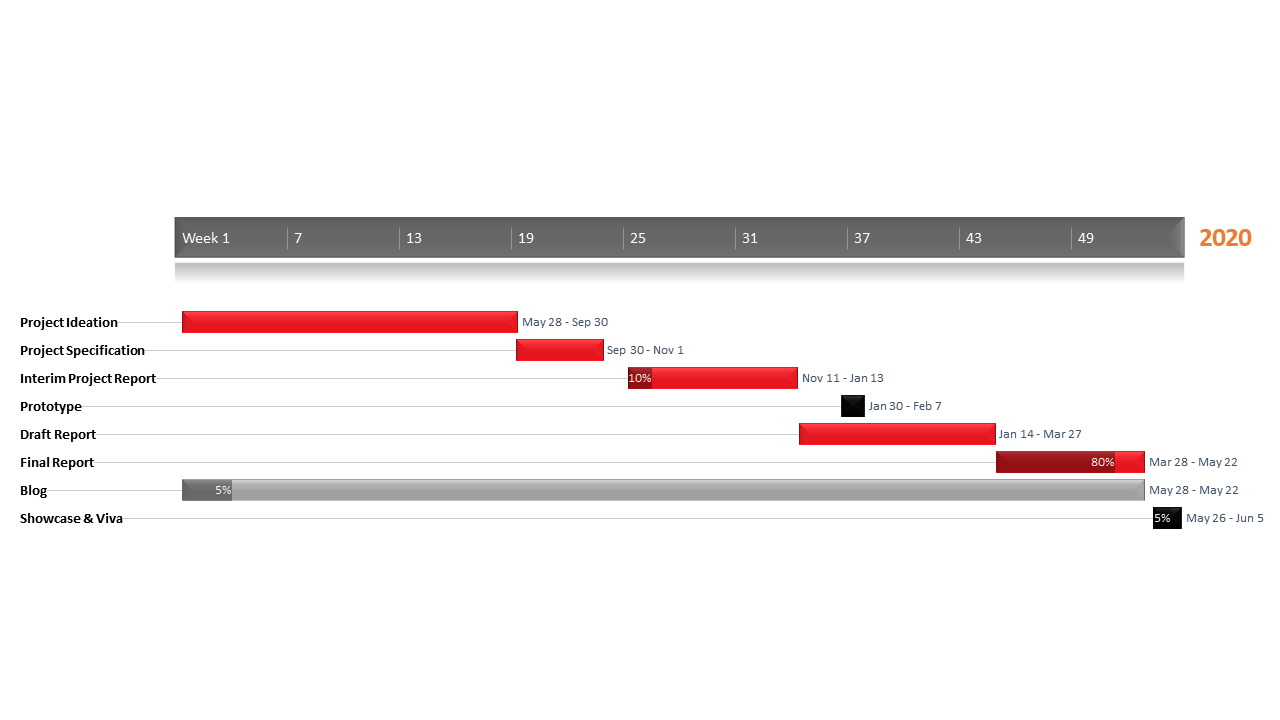
\includegraphics[width=6in]{/GanttChart.png}
				\caption[Gantt Chart]{Gantt Chart}
			\end{figure}
			
%-----------------------------------------------------------------------------------------------
%					END
%-----------------------------------------------------------------------------------------------
\chapter*{}
\vfill
\begin{center}
\textbf{END OF DOCUMENT}
\end{center}
\vfill
\end{document}